
\chapter{Τεχνικές Αύξησης της Διάρκειας Ζωής ενός ΑΔΑ}\label{ch:energy_reduction}


\section{Αποδοτικά Πρωτόκολλα Δρομολόγησης}
Η αποδοτική δρομολόγηση στα δίκτυα αισθητήρων αποτελεί ένα από τα πιο προκλητικά προβλήματα λόγω των ιδιαίτερων χαρακτηριστικών που τα διαχωρίζουν από τα κλασσικά
δίκτυα και ασύρματα δίκτυα αισθητήρων.
Καταρχήν πολλές φορές δεν είναι δυνατό να κτιστεί ένας καθολικός τρόπος διευθυνσιοδότησης λόγω του τεράστιου αριθμού των αισθητήρων.
Επομένως πρωτόκολλα τα οποία είναι βασισμένα στην διευθυνσιοδότηση IP δεν μπορούν να εφαρμοστούν στα δίκτυα αισθητήρων.
Δεύτερον, σε αντίθεση με τα κλασσικά δίκτυα δεδομένων, σχεδόν σε όλες τις εφαρμογές των ΑΔΑ απαιτούνται δεδομένα από πολλές διαφορετικές περιοχές ανίχνευσης τα
οποία προωθούνται σε μία συγκεκριμένη Πηγή.
Επιπλέον, στα δεδομένα που αναπαράγονται μπορεί να υπάρχει πλεονασμός πληροφορίας αφού πολλές μικρές περιοχές μπορεί να παράγουν τα ίδια δεδομένα.
Αυτός ο πλεονασμός πρέπει να εκμεταλλευθεί από τα πρωτόκολλα δρομολόγησης αποδοτικά έτσι ώστε να επιτευχθεί μείωση της κατανάλωσης της ενέργειας και επέκταση του
χρόνου ζωής του δικτύου.
Στην συνέχεια θα περιγραφούν συνοπτικά τα πιο γνωστά πρωτόκολλα δρομολόγησης.


\subsection{Δεδομένο-κεντρικά πρωτόκολλα}
Όπως αναφέρθηκε σε ορισμένες εφαρμογές δεν είναι δυνατόν να ορίσουμε ξεχωριστά αναγνωριστικά (IDs) σε κάθε κόμβο ενός ΑΔΑ κυρίως λόγω του αριθμού των κόμβων.
Αυτή η αδυναμία σε συνδυασμό με την τυχαία ανάπτυξη των κόμβων καθιστούν αδύνατη την επιλογή ενός υποσυνόλου κόμβων για την απαίτηση
συγκεκριμένων πληροφοριών (queries).
Επομένως τα δεδομένα συνήθως μεταδίδονται από κάθε κόμβο και υπάρχει σημαντικός πλεονασμός στην πληροφορία.
Επειδή ο πλεονασμός καταναλώνει μεγαλύτερη ενέργεια σε ένα ΑΔΑ, έχουν αναπτυχθεί δεδομένο-κεντρικά πρωτόκολλα δρομολόγησης τα οποία εκμεταλλεύονται τον πλεονασμό
πληροφορίας για να επιλέξουν υποσύνολα κόμβων. Τα πιο γνωστά δεδομενο-κεντρικά πρωτόκολλα δρομολόγησης είναι τα εξής:

\paragraph{Flooding και Gossiping:} Τα πρωτόκολλα πλημμύρας (flooding) και κουτσομπολιού (gossiping) \cite{gossiping} είναι δύο κλασσικοί μηχανισμοί για την μετάδοση
δεδομένων σε δίκτυα αισθητήρων χωρίς την χρήση κάποιου αλγορίθμου δρομολόγησης ή την συντήρηση κάποιας συγκεκριμένης τοπολογίας.
Στην μέθοδο πλημμύρας κάθε κόμβος μόλις λάβει ένα πακέτο δεδομένων το στέλνει σε όλους τους γείτονές του. Αυτή η διαδικασία συνεχίζεται μέχρι το πακέτο να φτάσει
στον προορισμό του ή όταν ο αριθμός των βημάτων (hops) που διήνυσε το πακέτο ξεπεράσει έναν συγκεκριμένο αριθμό (συνήθως την διάμετρο του δικτύου). Η μέθοδος του
κουτσομπολιού είναι μια λίγο πιο εξελιγμένη μορφή της μεθόδου πλημμύρας. Αντί ένας κόμβος, μόλις λάβει ένα καινούργιο πακέτο, να το στείλει σε όλους τους γείτονές
του,
το στέλνει σε έναν γείτονα ο οποίος επιλέγεται τυχαία, ομοιόμορφα κατανεμημένα, από το σύνολο των γειτόνων του.

Παρόλο που τα δύο αυτά πρωτόκολλα μπορούν να υλοποιηθούν πάρα πολύ εύκολα, έχουν αρκετά μειονεκτήματα σχετικά με την απόδοσή τους. Συγκεκριμένα, η μέθοδος
πλημμύρας έχει πολύ μεγάλο πλεονασμό δεδομένων και επομένως σπαταλάει την ενέργεια του δικτύου. Αντίθετα, η μέθοδος κουτσομπολιού έχει πολύ μεγάλη καθυστέρηση αφού ο
τρόπος που επιλέγονται οι επόμενοι κόμβοι είναι τυχαίος.

\paragraph{SPIN:} Το πρωτόκολλο SPIN (Sensor Protocols for Information via Negotiation) \cite{spin_protocol} είναι από τις πρώτες εργασίες που έγιναν με στόχο να
χρησιμοποιηθεί ένας δεδομενοκεντρικός μηχανισμός για την δρομολόγηση στα δίκτυα αισθητήρων. Η ιδέα πίσω από το πρωτόκολλο SPIN είναι να ονομάζει τα δεδομένα,
χρησιμοποιώντας υψηλού επιπέδου περιγραφείς (descriptors) και μετα-δεδομένα (meta-data). Πριν την αποστολή κάποιου πακέτου δεδομένων, τα μετα-δεδομένα ανταλλάσσονται
πρώτα ανάμεσα στους κόμβους μέσα από έναν μηχανισμό διαφήμισης. Κάθε κόμβος μόλις λάβει ένα νέο πακέτο δεδομένων το διαφημίζει σε όλους τους γείτονές του. Οι γείτονες
που ενδιαφέρονται, ζητάνε τα δεδομένα να τους αποσταλούν.

Ένα από τα πλεονεκτήματα του πρωτοκόλλου SPIN είναι ότι οι τοπολογικές αλλαγές είναι τοπικές αφού ο κάθε γείτονας χρειάζεται να ξέρει ουσιαστικά μόνο τους γείτονες
που είναι ένα βήμα (hop) μακριά. Επίσης η κατανάλωση ενέργειας μειώνεται κατά έναν παράγοντα 3.5 \cite{spin_protocol} σε σχέση με το πρωτόκολλο της πλημμύρας. Το
μειονέκτημα του πρωτοκόλλου είναι ότι ο μηχανισμός διαφήμισης που χρησιμοποιεί δεν επαρκεί για να υπάρχει κάποια εγγύηση στην παράδοση δεδομένων. Διότι αν ένας κόμβος
που ενδιαφέρεται στα δεδομένα είναι πολύ μακριά απ τον κόμβο που τα παράγει τότε όλοι οι κόμβοι που βρίσκονται στο ενδιάμεσο δεν ενδιαφέρονται και επομένως τα
δεδομένα πολύ πιθανόν να μην παραδοθούν καθόλου στον προορισμό τους.

\paragraph{Directed Diffusion:}  Το πρωτόκολλο Directed Diffusion (DD) \cite{directed_diffusion} αποτελεί ένα σημαντικό ορόσημο στα δεδομενο-κεντρικά πρωτόκολλα και
στην έρευνα των δικτύων αισθητήρων. Η ιδέα στοχεύει στη διάχυση δεδομένων μέσα από τους κόμβους χρησιμοποιώντας ένα σχήμα ονομασίας για τα δεδομένα. Ο κύριος λόγος
για την χρησιμοποίηση ενός τέτοιου σχήματος είναι για να ξεφορτωθεί το πρωτόκολλο δρομολόγησης από άχρηστες εργασίες χαμηλότερων επιπέδων έτσι ώστε να εξοικονομηθεί
ενέργεια. Το πρωτόκολλο χρησιμοποιεί ζευγάρια ιδιότητας-τιμής σε αναθέσεις επερωτημάτων (queries). Προκειμένου να γίνει ένα επερώτημα, ένα "ενδιαφέρον" (interest)
ορίζεται χρησιμοποιώντας μια λίστα από τέτοια ζευγάρια όπως για παράδειγμα ονόματα αντικειμένων, διάστημα, διάρκεια, γεωγραφική περιοχή και άλλα. Το "ενδιαφέρον"
μεταδίδεται από την Πηγή προς όλες τις κατευθύνσεις (broadcast). Κάθε κόμβος αφού λάβει ένα "ενδιαφέρον" το αποθηκεύει στη μνήμη του για όσο καιρό είναι έγκυρο. Τα
"ενδιαφέροντα" στην μνήμη χρησιμοποιούνται για να συγκριθούν με τα ληφθέντα δεδομένα που έχουν τις συγκεκριμένες ιδιότητες και τιμές. Επίσης κάθε "ενδιαφέρον" έχει
κάποια επιπλέον πεδία που αφορούν τους συνδέσμους ανάμεσα σε έναν κόμβο και τους γείτονες που απάντησαν με δεδομένα σχετικά με το ενδιαφέρον. Τέτοια πεδία είναι η
ποιότητα του συνδέσμου, ο ρυθμός των εισερχόμενων δεδομένων η διάρκεια κ.α. Επομένως χρησιμοποιώντας αυτούς τους μηχανισμούς μπορούν να εγκατασταθούν πραγματικά
μονοπάτια μεταξύ των κόμβων που παράγουν δεδομένα και της Πηγής. Η Πηγή στο τέλος ξαναστέλνει το αυθεντικό πακέτο "ενδιαφέρον" χρησιμοποιώντας τα καινούργια
μονοπάτια. Με αυτόν τον τρόπο ουσιαστικά ενισχύει τα μονοπάτια αυτά τα οποία με μεγάλη πιθανότητα είναι και τα καλύτερα. Ένα παράδειγμα φαίνεται στην εικόνα
\ref{fig:dd_example}

\begin{figure}[h]
	\centering
	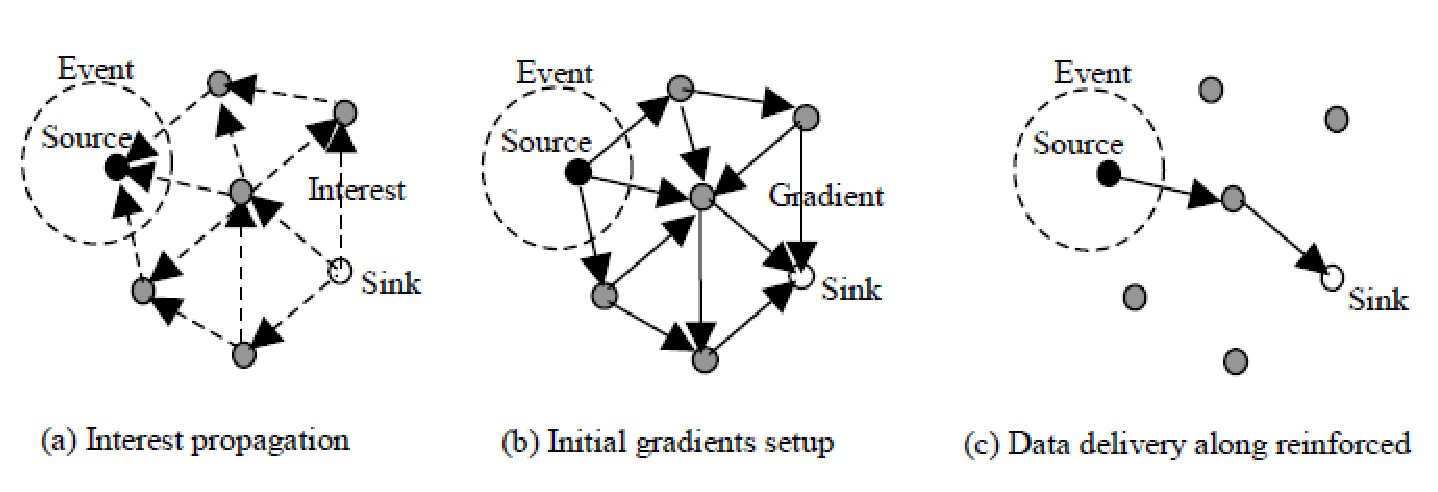
\includegraphics[width=\textwidth]{images/directed_diffusion.eps}
	\caption{Ένα σενάριο του πρωτοκόλλου Directed Diffusion.}
	\label{fig:dd_example}
\end{figure}

Το πρωτόκολλο Directed Diffusion διαφέρει από το SPIN ως προς το τρόπο που ζητάει τις πληροφορίες, δηλαδή τον τρόπο που θέτει τα επερωτήματα. Στο DD η Πηγή θέτει
επερώτημα σε όλους τους αισθητήρες αν κάποια συγκεκριμένα δεδομένα είναι διαθέσιμα. Αν υπάρχουν τα δεδομένα ανάλογα με τα μονοπάτια που έχουν δημιουργηθεί, αυτά
ενισχύονται από την Πηγή. Αντίθετα στο SPIN κάθε κόμβος διαφημίζει τα δεδομένα του στους υπόλοιπους κόμβους. Εάν κάποιος κόμβος ενδιαφέρεται τότε τα απαιτεί. Είναι
εμφανές ότι στο πρωτόκολλο DD υπάρχει υπεροχή όσον αφορά στην εξοικονόμηση ενέργειας ειδικά αν τα γεγονότα που εμφανίζονται στο δίκτυο έχουν μεγάλη διάρκεια. Όμως αν
τα γεγονότα έχουν πολύ μικρή διάρκεια τότε το DD έχει πολύ μικρή απόδοση αφού η κατανάλωση (overhead) που θα υπάρχει μέχρι να στηθούν τα μονοπάτια θα είναι
συγκρίσιμη με την ενέργεια που σπαταλάται για να μεταφερθούν τα πραγματικά δεδομένα.

\paragraph{Rumor routing:} Η δρομολόγηση ανά φήμες (rumor routing) \cite{rumor_routing} είναι μια παραλλαγή του πρωτοκόλλου Directed Diffusion και έχει κυρίως να
κάνει
με ΑΔΑ στα οποία γεωγραφικά κριτήρια δεν μπορούν να εφαρμοστούν. Γενικώς το DD πλημμυρίζει το δίκτυο με πακέτα προς όλους τους κόμβους μέχρι να φτιαχτούν τα
πραγματικά μονοπάτια τα οποία θα εμπεριέχουν ένα πολύ μικρό ποσοστό των συνολικών κόμβων του δικτύου. Αντίθετα στην δρομολόγηση ανά φήμες ο κάθε κόμβος προωθεί το
αναγνωριστικό πακέτο μόνο αν έχει "ακούσει" και ο ίδιος κάτι. Προσομοιώσεις έχουν δείξει ότι με αυτόν τον τρόπο εξοικονομείται περισσότερη ενέργεια στο δίκτυο
αισθητήρων μόνο όταν ο αριθμός των γεγονότων είναι σχετικά μικρός.

\paragraph{COUGAR:} Αυτό το δεδομενο-κεντρικό πρωτόκολλο είναι ριζοσπαστικό σε σχέση με τα υπόλοιπα καθώς βλέπει όλο το δίκτυο ως μια τεράστια, κατανεμημένη, βάση
δεδομένων \cite{cougar_protocol}. Η βασική ιδέα είναι να χρησιμοποιεί δηλωτικά ερωτήματα (declarative queries) με σκοπό να δημιουργήσει αφηρημένα επερωτήματα όπως η
επιλογή όλων των σχετικών κόμβων με μια πληροφορία κλπ. Αυτή η αφαίρεση γίνεται μέσα από ένα καινούργιο επίπεδο, αυτό των επερωτημάτων ανάμεσα στο επίπεδο δικτύου και
το επίπεδο των εφαρμογών. Όμως παρόλο που το επίπεδο αυτό είναι ανεξάρτητο του δικτύου έχει κάποια μειονεκτήματα. Καταρχήν ένα επιπλέον επίπεδο στην στοίβα του
δικτύου θα καταναλώνει περισσότερη ενέργεια σε κάθε κόμβο. Επιπλέον, όπως και στις πραγματικές κατανεμημένες βάσεις δεδομένων, έτσι και εδώ θα πρέπει να λύνονται
αποδοτικά θέματα συγχρονισμού.

\subsection{Ιεραρχικά Πρωτόκολλα}
Όπως και στα κλασσικά δίκτυα ένα από τα πιο σημαντικά ζητήματα σχεδιασμού είναι αυτό της κλιμακωσιμότητας. Ένα "επίπεδο" δίκτυο μπορεί να προκαλέσει στην πύλη
δικτύου (gateway) υπερφόρτωση όταν το μέγεθος του δικτύου γίνει πολύ μεγάλο. Κατά συνέπεια η υπερφόρτωση μπορεί να προκαλέσει σοβαρή καθυστέρηση στις επικοινωνίες
και αντίστοιχα να χαθούν μερικά γεγονότα ή οι χρονικοί περιορισμοί που ορίζονται από αυτά. Ειδικά στην περίπτωση των ΑΔΑ όπου ο κάθε κόμβος έχει πολύ μικρή ακτίνα
εμβέλειας, η κλιμακωσιμότητα ενός "επίπεδου" πρωτοκόλλου δρομολόγησης είναι πολύ δύσκολη. Το πρόβλημα μπορεί να λυθεί εισάγοντας την έννοια της ιεραρχίας που πολλές
φορές γίνεται με μικρές συστάδες (clusters) σε όλη την περιοχή του δικτύου. Σε κάθε συστάδα συνήθως εκλέγεται ένας αρχηγός (cluster head) ο οποίος είναι υπεύθυνος για
την συστάδα του. Τα μέλη της συστάδας, κόμβοι του ΑΔΑ, ορίζονται από την ακτίνα εμβέλειας του αρχηγού όταν αυτός εκπέμψει ένα αναγνωριστικό μήνυμα. Αν σε έναν κόμβο
έρθει παραπάνω από ένα αναγνωριστικά μηνύματα τότε ο κόμβος θα γίνει μέλος της συστάδας της οποία το αναγνωριστικό σήμα είχε το καλύτερο (δυνατότερο) σήμα. Στην
συνέχεια παρουσιάζονται τα πιο γνωστά ιεραρχικά πρωτόκολλα δρομολόγησης.

\paragraph{LEACH:} Το πρωτόκολλο LEACH (Low-Energy Adaptive Clustering Hierarchy) \cite{leach_protocol} είναι ένα από τα πιο γνωστά ιεραρχικά πρωτόκολλα δρομολόγησης
για δίκτυα αισθητήρων. Η βασική ιδέα είναι να δημιουργηθούν συστάδες (clusters) βάση την ισχύ του ληφθέντος σήματος από τον αρχηγό. Οι κόμβοι της κάθε συστάδας,
χρησιμοποιώντας πολυ-βηματικές (multi-hop) μεταδόσεις, στέλνουν τα δεδομένα τους στον αρχηγό ο οποίος τα μαζεύει και τα στέλνει απευθείας στην Πηγή. Με αυτόν τον
τρόπο μειώνεται η κατανάλωση της ενέργειας αφού μόνο οι αρχηγοί κάνουν μακρινές μεταδόσεις δεδομένων. Έχει υπολογιστεί ότι ο βέλτιστος αριθμός αρχηγών σε ένα δίκτυο
είναι περίπου το 5\% όλων των κόμβων του δικτύου. Προκειμένου να υπάρχει ακόμη μεγαλύτερη ισορροπία στην ενέργεια, οι αρχηγοί και κατά συνέπεια και οι συστάδες,
αλλάζουν ανά τακτά χρονικά διαστήματα. Συγκεκριμένα ένας κόμβος γίνεται αρχηγός με την παρακάτω πιθανότητα:

\begin{align*}
T(n) = \left\{
\begin{array}{cc}
 \frac{p}{1-p\cdot(r \text{mod}\frac{1}{p})} & \text{if } x<0 \\
  0 & \text{αλλιώς}
\end{array} \right.
\end{align*}
όπου $p$ είναι το επιθυμητό ποσοστό των αρχηγών, $r$ είναι ο τρέχον γύρος και G είναι το σύνολο των κόμβων που δεν έχουν γίνει αρχηγοί τους προηγούμενους
$\frac{1}{p}$
γύρους.

Το πρωτόκολλο LEACH μπορεί να πετύχει μέχρι και 7 φορές λιγότερη κατανάλωση ενέργειας σε σχέση με τα κλασσικά πρωτόκολλα ασύρματων δικτύων \cite{leach_protocol} ενώ
ακόμα και 12 χρόνια μετά την δημοσίευσή του παραμένει ένα από τα πιο κλασσικά πρωτόκολλα ΑΔΑ. Τα μόνα μειονεκτήματά του (τα οποία βελτιώθηκαν από επόμενες
δημοσιεύσεις) είναι ότι το μοντέλο που υποθέτει για την ακτίνα εμβέλειας των κόμβων, για πολύ μεγάλα δίκτυα, είναι μη ρεαλιστικό. Επίσης, για πολύ μεγάλα δίκτυα οι
αρχηγοί των συστάδων που βρίσκονται πολύ μακριά από την Πηγή εξαντλούν πολύ πιο γρήγορα την ενέργειά τους απ'ότι οι αρχηγοί των συστάδων που βρίσκονται κοντά στην
Πηγή.

\paragraph{PEGASIS \& Hierarchical-PEGASIS:} Το πρωτόκολλο PEGASIS (Power-Efficient Gathering in Sensor Information Systems) \cite{pegasis_protocol} αποτελεί μια
βελτίωση του πρωτοκόλλου δρομολόγησης LEACH. Αντί να δημιουργούνται συστάδες, το PEGASIS σχηματίζει αλυσίδες με όλους τους κόμβους έτσι ώστε κάθε κόμβος λαμβάνει μόνο
από έναν κόμβο και αφού ενσωματώσει και τα δικά του δεδομένα τα αποστέλλει σε μόνον έναν γείτονα. Ταυτόχρονα μόνο ένας κόμβος στην αλυσίδα έχει επιλεχτεί τυχαία ως
αρχηγός ο οποίος αναλαμβάνει να μαζέψει όλα τα δεδομένα και τα αποστέλλει στην Πηγή. Η διαφορά από το LEACH είναι ότι χρησιμοποιεί πολυ-βηματικές (multi-hop)
μεταδόσεις μεταξύ των κόμβων και ότι μόνο ένας κόμβος σε κάθε γύρο είναι ο αρχηγός που αποστέλλει τα δεδομένα στην Πηγή. Προσομοιώσεις δείξαν ότι μπορεί να βελτιώσει
ακόμα και 100\% την εξοικονόμηση ενέργειας σε σχέση με το LEACH. Το αρνητικό του όμως είναι ότι μπορεί τα πακέτα να έχουν μεγάλη καθυστέρηση μέχρι να φτάσουν στην
Πηγή. Το πρωτόκολλο Hierarchical-PEGASIS \cite{hierarchical_pegasis} αποτελεί μια προέκταση του PEGASIS το οποίο σκοπεύει στην μείωση της καθυστέρησης που
παρουσιάζεται στο PEGASIS. Ουσιαστικά δημιουργούνται περισσότερες από μια αλυσίδες με τον ίδιο προορισμό. Επίσης για την δημιουργία της αλυσίδας εφαρμόζει την μετρική
$energy\times delay$.

\paragraph{TEEN \& APTEEN:} Το πρωτόκολλο TEEN (The Energy Efficient sensor Network protocol) \cite{teen_protocol} είναι ένα
ιεραρχικό πρωτόκολλο σχεδιασμένο να μπορεί να ανταποκρίνεται γρήγορα στις γρήγορες αλλαγές όπως είναι η θερμοκρασία με μεγάλη λεπτομέρεια. Η γρήγορη ανταπόκριση είναι
σημαντικό στοιχείο σε δίκτυα πραγματικού χρόνου. Οι συστάδες (clusters) σχηματίζονται παρόμοια με το LEACH πρωτόκολλο αλλά για για να πετύχει την γρήγορη ανταπόκριση,
το πρωτόκολλο ορίζει δύο κατώφλια που έχουν σχέση με τον τρόπο ανίχνευσης των γεγονότων από τους κόμβους. Το πρώτο ονομάζεται το σκληρό κατώφλι (hard threshold) και
ορίζει τις μικρότερες δυνατές τιμές μιας ιδιότητας που θα κάνουν τον κόμβο να "ξυπνήσει", δηλαδή να επανέλθει σε κανονική λειτουργία και να ενεργοποιήσει τον μεταδότη
του. Επομένως το σκληρό κατώφλι επιτρέπει τον κάθε κόμβο να αναφέρει δεδομένα μόνο όταν οι ιδιότητες αυτών ξεπεράσουν μια συγκεκριμένη τιμή που έχει να κάνει με το
πόσο ενδιαφέρον έχουν τα δεδομένα. Αντίθετα το μαλακό κατώφλι (soft threshold) επιτρέπει την μετάδοση δεδομένων μόνο όταν το ποσοστό των αλλαγών ξεπεράσουν την τιμή
του μαλακού κατωφλίου. Έτσι μειώνονται ακόμα περισσότερο οι μεταδόσεις πακέτων οι οποίες αφορούν πολύ μικρές αλλαγές στην περιοχή αίσθησης του κόμβου. Το μόνο
πρόβλημα που αντιμετωπίζει το πρωτόκολλο TEEN είναι όταν ο διαχειριστής του δικτύου επιθυμεί ο κάθε κόμβος να επιστρέφει πληροφορίες σε περιοδικό χρόνο. Το πρόβλημα
αυτό λύθηκε από μια προέκταση του TEEN, το ATEEN (Adaptive TEEN) \cite{apteen_protocol} στο οποίο μπορεί να ορίσει η Πηγή με ποιον τρόπο θα γίνονται οι αναφορές από
κάθε κόμβο.


\subsection{Πρωτόκολλα Βασισμένα στην Τοποθεσία}
Πολλές φορές πρωτόκολλα για τα ΑΔΑ απαιτούν πληροφορίες για την τοποθεσία για τους κόμβους.
Στις περισσότερες περιπτώσεις οι πληροφορίες αυτές χρειάζονται για να υπολογιστούν οι αποστάσεις μεταξύ κόμβων και να εκτιμηθεί η ενέργεια που χρειάζεται για να
αποσταλεί ένα πακέτο.
Επιπλέον, εφόσον δεν εφαρμόζονται πρωτόκολλα βασισμένα στην διευθυνσιοδότηση IP για τα δίκτυα αισθητήρων όπως συμβαίνει στα κλασσικά δίκτυα δεδομένων, ενώ ταυτόχρονα
οι κόμβοι είναι όλοι τοποθετημένοι σε μια συγκεκριμένη γεωγραφική περιοχή, πληροφορίες για την συγκεκριμένη τοποθεσία τους μέσα στην γεωγραφική περιοχή μπορούν
να χρησιμοποιηθούν για την δρομολόγηση δεδομένων και την μείωση της κατανάλωσης της ενέργειας.
Για παράδειγμα, αν η περιοχή που πρέπει να επιβλεφθεί για συγκεκριμένο σκοπό είναι γνωστή, χρησιμοποιώντας τις πληροφορίες τοποθεσίας των κόμβων, το επερώτημα (query)
προς το δίκτυο μπορεί να διοχετευθεί σε συγκεκριμένους κόμβους μόνο.
Αν και έχουν αναπτυχθεί αρκετά πρωτόκολλα τοπολογικής δρομολόγησης για τα κλασσικά ασύρματα δίκτυα αισθητήρων, αυτά δεν είναι εφαρμόσιμα στα ΑΔΑ καθώς η μετρική
απόδοσης που έχουν δεν περιλαμβάνει την μείωση της καταναλισκόμενης ενέργειας. Παρακάτω παρουσιάζονται τα πιο γνωστά πρωτόκολλα δρομολόγησης που βασίζονται στην
τοπολογία.


\paragraph{GAF:} Το πρωτόκολλο GAF (Geographic Adaptive Fidelity) \cite{gaf_protocol} είναι ένας ενεργειακός και βασισμένος στην τοπολογία αλγόριθμος δρομολόγησης
σχεδιασμένος αρχικά για ασύρματα δίκτυα αλλά πλέον εφαρμόζεται και σε ασύρματα δίκτυα αισθητήρων. Ο αλγόριθμος αυτός, εξοικονομεί ενέργεια απενεργοποιώντας περιττούς
κόμβους χωρίς να επηρεάζει την ποιότητα δρομολόγησης του δικτύου. Ο αλγόριθμος δημιουργεί ένα εικονικό πλέγμα (grid) για την περιοχή που καλύπτεται. Κάθε κόμβος
χρησιμοποιεί την τοποθεσία του για να συσχετίσει τον εαυτό του με κάποιο σημείο (τετράγωνο) του πλέγματος. Οι κόμβοι που είναι συσχετισμένοι με το ίδιο σημείο στο
πλέγμα θεωρούνται ότι είναι ισοδύναμοι όσον αφορά το κόστος της δρομολόγησης. Αυτή η ισοδυναμία εκμεταλλεύεται απενεργοποιώντας μερικούς κόμβους και αφήνοντας μόνο
έναν ενεργοποιημένο σε κάθε σημείο (τετραγωνάκι) του πλέγματος. Ένα παράδειγμα φαίνεται στην εικόνα \ref{fig:gaf_example}. Συγκεκριμένα ο κόμβος 1 μπορεί να
επικοινωνήσει τους 2,3 και 4 και οι κόμβοι 2,3 και 4 μπορούν να επικοινωνήσουν με τον κόμβο 5. Επομένως οι κόμβοι 2,3 και 4 είναι ισοδύναμοι και οι δύο από αυτούς
μπορούν να απενεργοποιηθούν εξοικονομώντας ενέργεια.

\begin{figure}[h]
	\centering
	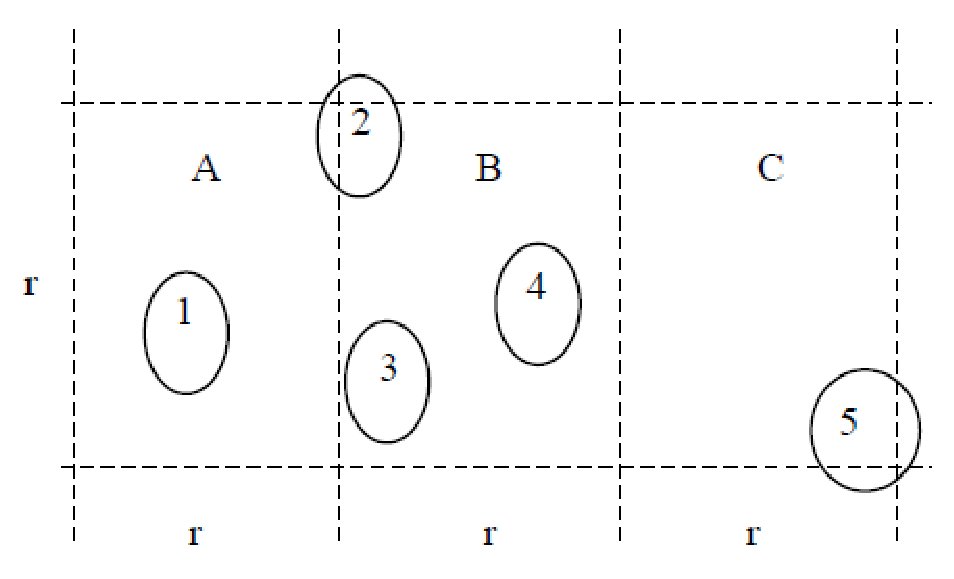
\includegraphics[width=0.6\textwidth]{images/gaf_example.eps}
	\caption{Ένα σενάριο του πρωτοκόλλου GAF.}
	\label{fig:gaf_example}
\end{figure}

Οι εξομοιώσεις έχουν δείξει ότι το πρωτόκολλο GAF μπορεί να έχει την ίδια απόδοση όσον αφορά την χρονοκαθυστέρηση (latency) και την απώλεια πακέτων σε σχέση με τα
κλασσικά πρωτόκολλα ασύρματων δικτύων, ενώ ταυτόχρονα αυξάνει την διάρκεια ζωής του δικτύου σε σημαντικό βαθμό.

\paragraph{GEAR:} Το πρωτόκολλο GEAR (Geographical and Energy Aware Routing) \cite{gear_protocol} προτείνει την χρησιμοποίηση γεωγραφικών δεδομένων για την διάδοση
επερωτημάτων για συγκεκριμένες περιοχές αφού στις επερωτήσεις πολύ συχνά ενσωματώνονται γεωγραφικές ιδιότητες. Το πρωτόκολλο χρησιμοποιεί ενεργειακές και γεωγραφικές
ευρετικές μεθόδους προκειμένου να δρομολογήσει κάποιο πακέτο. Η ιδέα είναι να περιορίσει τον αριθμό των πακέτων "ενδιαφέροντος" που χρησιμοποιεί το πρωτόκολλο
Directed Diffusion \cite{directed_diffusion} θεωρώντας μόνο μια συγκεκριμένη περιοχή και όχι όλη την περιοχή του δικτύου. Στο πρωτόκολλο GEAR, κάθε κόμβος κρατάει
ένα κόστος εκτίμησης και ένα κόστος μάθησης της διαδρομής του πακέτου μέχρι τον προορισμό. Το κόστος εκτίμησης είναι ένας συνδυασμός της υπολειπόμενης ενέργειας και
της απόστασης μέχρι τον προορισμό. Το κόστος μάθησης είναι ουσιαστικά το κόστος εκτίμησης αλλά λαμβάνει υπόψιν και της ενεργειακές τρύπες του δικτύου που συμβαίνουν
όταν ένας κόμβος δεν έχει κανένα κοντινότερο γείτονα προς τον προορισμό εκτός από τον εαυτό του. Το κόστος μάθησης διαδίδεται ένα βήμα (hop) μακριά κάθε φορά που ένα
πακέτο φτάνει στον προορισμό του έτσι ώστε να χρησιμοποιηθεί στην επόμενη δρομολόγηση.


% \paragraph{GPSR:} Το πρωτόκολλο GPSR (Greedy Perimeter Stateless Routing for Wireless Networks)


\subsection{Πρωτόκολλα Εξισορρόπησης Ενέργειας}
Όλα τα προηγούμενα πρωτόκολλα είχαν στόχο την μείωση της κατανάλωσης του δικτύου αισθητήρων και ως απώτερο σκοπό την επέκταση της διάρκειας ζωής του δικτύου.
Όμως πολλά από αυτά τα πρωτόκολλα δημιουργούν "παρενέργειες" σε ένα ΑΔΑ.
Για παράδειγμα στο πρωτόκολλο LEACH \cite{leach_protocol} οι αρχηγοί των συστάδων στέλνουν τα δεδομένα τους κατευθείαν στην Πηγή. Όμως οι αρχηγοί των συστάδων οι
οποίες βρίσκονται στην άκρη του δικτύου, δηλαδή μακριά από την Πηγή έχουν πολύ μεγαλύτερο κόστος μετάδοσης από ότι οι αρχηγοί των συστάδων που βρίσκονται κοντά στην
Πηγή.
Επομένως οι κόμβοι που βρίσκονται μακριά από την Πηγή εξαντλούν πολύ γρηγορότερα την ενέργειά τους και ενώ το δίκτυο συνεχίζει τη λειτουργία του, ένα κομμάτι
του δεν επιβλέπεται.
Ενα παρόμοιο παράδειγμα είναι το πρωτόκολλο Directed Diffusion \cite{directed_diffusion} όπου αφού φτιαχτούν τα μονοπάτια, δημιουργείται μια δενδρική δομή με ρίζα την
Πηγή όπου όλοι οι κόμβοι στέλνουν προς την Πηγή.
Είναι επομένως λογικό ότι οι κόμβοι που είναι κοντά στην Πηγή, αντιμετωπίζουν ένα πολύ μεγαλύτερο φορτίο σε σχέση με τους κόμβους που είναι μακριά από την αυτή.
Ένα παράδειγμα φαίνεται στην εικόνα \ref{fig:energy_holes}.

\begin{figure}[h]
	\centering
	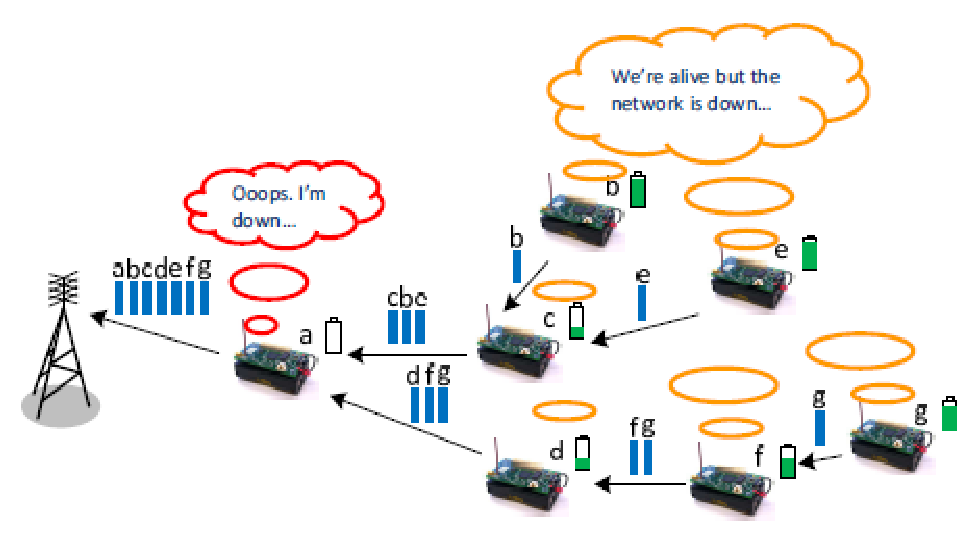
\includegraphics[width=0.8\textwidth]{images/energy_holes.eps}
	\caption{Ένα παράδειγμα υπερφόρτωσης των κόμβων κοντά στην Πηγή}
	\label{fig:energy_holes}
\end{figure}

Λόγω αυτής της υπερφόρτωσης των κόμβων κοντά στην Πηγή, οι κόμβοι αυτοί αποφορτίζονται πολύ πιο γρήγορα από ότι οι κόμβοι μακριά από την
Πηγή. Έτσι μετά από μικρό χρονικό διάστημα λειτουργίας του δικτύου οι κόμβοι αυτοί πεθαίνουν και δημιουργούνται μικρές ενεργειακές τρύπες (energy holes). Αυτό
δημιουργεί πρόβλημα στο δίκτυο καθώς αν όλοι οι κόμβοι κοντά στην Πηγή αποφορτιστούν πλήρως, τότε ουσιαστικά το δίκτυο καθίσταται άχρηστο καθώς οι κόμβοι που είναι
λίγο πιο μακριά από την Πηγή δεν μπορούν να στείλουν τα δεδομένα τους σε αυτήν. Μάλιστα, έχει δειχθεί ότι σε πρωτόκολλα όπως το Directed Diffusion όταν οι κόμβοι
κοντά στην Πηγή πεθάνουν, το δίκτυο έχει ακόμα το 90\% της ενέργειας του \cite{energy_holes}, όπου το μεγαλύτερο μέρος αυτής είναι κατανεμημένο στους κόμβους που
βρίσκονται στην άκρη του δικτύου. Αυτό σημαίνει ότι δεν υπάρχει αποδοτική διαχείριση της ενέργειας σε αυτά τα πρωτόκολλα. Η λύση σε αυτό το πρόβλημα δίνεται από
αλγόριθμους εξισορρόπησης ενέργειας.

Τα πρωτόκολλα εξισορρόπησης ενέργειας αυτό που προσπαθούν να κάνουν είναι, σε κάθε χρονική στιγμή, όλοι οι κόμβοι του δικτύου να έχουν περίπου την ίδια ενέργεια.
Είναι προφανές ότι τα πρωτόκολλα εξισορρόπησης ενέργειας καταναλώνουν περισσότερη ενέργεια από ότι τα πρωτόκολλα μείωσης της κατανάλωσης ενέργειας. Όμως η διάρκεια
ζωής\footnote{διάρκεια ζωής εννοούμε το χρονικό διάστημα μέχρι το δίκτυο να γίνει άχρηστο.} ενός ΑΔΑ αυξάνεται σημαντικά με τα πρωτόκολλα εξισορρόπησης ενέργειας
αφού σχεδόν όλοι οι κόμβοι είναι ενεργοί καθόλη τη διάρκεια της ζωής του δικτύου ενώ πεθαίνουν όλοι σχεδόν ταυτόχρονα προς το τέλος της. Υπάρχει πολύ μεγάλη έρευνα
για την εξισορρόπηση ενέργειας στα ασύρματα δίκτυα αισθητήρων ακόμα και σήμερα. Τα πιο σημαντικά πρωτόκολλα
εξισορρόπησης ενέργειας παρουσιάζονται παρακάτω:

\paragraph{EBP:} Το πρωτόκολλο EBP (Energy Balanced Protocol) \cite{ebp_protocol} είναι από τα πρώτα πρωτόκολλα εξισορρόπησης ενέργειας το οποίο έθεσε τις βάσεις του
προβλήματος και πρότεινε έναν πιθανοτικό αλγόριθμο. Συγκεκριμένα, το δίκτυο χωρίζεται σε $n$ δακτυλίους (ή τομείς), πλάτους $R$ ενώ η γωνία που καλύπτει το δίκτυο
θεωρείται ότι είναι $\phi$ όπως φαίνεται στην εικόνα \ref{fig:ebp_ring}.

\begin{figure}[h]
	\centering
	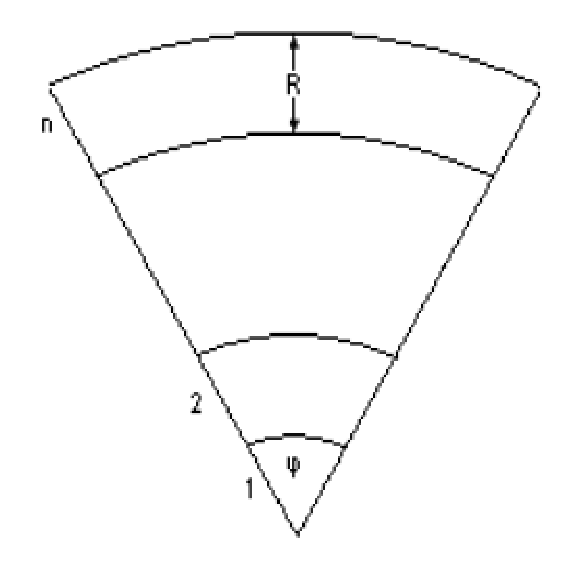
\includegraphics[width=0.4\textwidth]{images/ebp_ring.eps}
	\caption{Δίκτυο αισθητήρων με $n$ δακτυλίδια, γωνία $\phi$ και πλάτος δακτυλίου $R$}
	\label{fig:ebp_ring}
\end{figure}

Για την μετάδοση των πακέτων κάθε κόμβος στον δακτύλιο $i$ χρησιμοποιείται το εξής σχήμα:
\begin{itemize}
\item Μετάδωσε το πακέτο στον δακτύλιο $i-1$ με πιθανότητα $p_{i}$
\item Μετάδωσε το πακέτο απευθείας στην Πηγή με πιθανότητα $1-p_{i}$
\end{itemize}

Η επιλογή του $p_{i}$ γίνεται με τέτοιο τρόπο ώστε η μέση κατανάλωση ενέργειας κόμβου να είναι ίδια για όλους τους κόμβους στο δίκτυο.
Μετά από μία εκτενή ανάλυση οι συγγραφείς καταλήγουν στον παρακάτω τύπο:
\begin{align*}
p_{i} = \frac{E[f_{i}]}{E[f_{i+1}] + E[g_{i+1}]}
\end{align*}
όπου $E[f_{i}]$ είναι η μέση τιμή των μηνυμάτων που προωθούνται στον δακτύλιο $i$ και
\begin{align*}
E[f_{i}] = - \sum\limits^{n-i}_{k=1}\frac{\prod_{j=k}^{n-i+1}\alpha(n-j)}{\prod_{j=k}^{n-i}d(n-j)}\cdot
\left(\sum\limits_{j=1}^{n-k}(a(j)E[g_{j}]-\alpha(j+1)E[g_{j+1}])+\alpha(1)\cdot E[f_{1}]\right)
\end{align*}
ενώ $E[g_{i}]$ η μέση τιμή των μηνυμάτων που παράγονται και καθορίζονται από το δίκτυο.

Κάνοντας την παραδοχή ότι $E[f_{i}] \approx E[f_{i+1}]$, ότι δηλαδή τα μηνύματα που προωθούνται στον δακτύλιο $i$ είναι περίπου ίσα με τα μηνύματα που προωθούνται
στον δακτύλιο $i+1$ τότε δημιουργείται ο εξής κλειστός προσεγγιστικός τύπος για τις πιθανότητες $p_{i}$:
\begin{align*}
p_{i} = \frac{3x}{(i+1)(i-1)}
\end{align*}
όπου $p_{2} = x \in (0,1)$ είναι παραμετροποιήσιμη μεταβλητή ενώ $p_{1} =0$.

Όταν το $i$ είναι μεγάλο τότε και η πιθανότητα $p_{i}$ είναι μεγάλη. Αυτό συμβαίνει γιατί όταν ένας κόμβος είναι μακριά από την Πηγή τότε είναι
καλύτερα να στέλνει βήμα-βήμα (hop by hop) για να αποφύγει να σπαταλήσει μεγάλη ενέργεια για την αποστολή απευθείας στην Πηγή. Αντίθετα, όταν το $i$ είναι μικρό τότε
η πιθανότητα $p_{i}$ είναι μικρή.

\paragraph{Distributed EBP} Η εργασία στο \cite{debp_protocol} είναι μια επέκταση του πρωτοκόλλου EBP. Αρχικά
ορίζεται ως μικτή στρατηγική την δυνατότητα κάθε κόμβου να μπορεί να στείλει είτε στον αμέσως επόμενο γείτονά του είστε απευθείας στην Πηγή όπως στο EBP.
Αποδεικνύεται ότι οι μικτές στρατηγικές είναι οι βέλτιστες σε σχέση με οποιαδήποτε άλλη στρατηγική μετάδοσης των πακέτων. Στην συνέχεια κατασκευάζεται ένας τυφλός
άμεσης απόκρισης κατανεμημένος αλγόριθμος (blind, online distributed algorithm) ο οποίος λύνει το πρόβλημα της εξισορρόπησης της ενέργειας. Ο αλγόριθμος λειτουργεί ως
εξής:
\begin{itemize}
\item Αρχικά κάθε κόμβος ξέρει όλους τους γείτονές του και την εναπομείνασα ενέργειά τους
\item Κάθε κόμβος που θέλει να στείλει ένα πακέτο βρίσκει τον γείτονα με την χαμηλότερη εναπομείνασα ενέργεια έστω $n_{l}$
	\begin{itemize}
	\item Αν η εναπομείνασα ενέργεια του $n_{l}$ είναι μεγαλύτερη από την εναπομείνασα ενέργεια του κόμβου που θέλει να στείλει το πακέτο τότε το στέλνει στον
$n_{l}$
	\item Αντίθετα αν η εναπομείνασα ενέργεια του $n_{l}$ είναι μικρότερη τότε ο κόμβος που θέλει να στείλει το πακέτο το στέλνει απευθείας στην Πηγή
	\end{itemize}
\end{itemize}

Όπως φαίνεται ο αλγόριθμος χρησιμοποιεί μικτή στρατηγική όπως ο EBP, αλλά είναι κατανεμημένος και χρησιμοποιεί μόνο τοπική πληροφορία, σε αντίθεση με τον EBP.
Εξομοιώσεις δείξαν ότι ο αλγόριθμος μπορεί να εξισορροπήσει σχεδόν τέλεια την ενέργεια σε ένα ασύρματο δίκτυο αισθητήρων.

\paragraph{Offline EBP} H εργασίες στα \cite{oebp_protocol1} και \cite{oebp_protocol2} προσπαθούν να λύσουν το πρόβλημα της εξισορρόπησης ενέργειας από μια
διαφορετική σκοπιά. Η πρώτη εργασία εξετάζει την περίπτωση ομοιόμορφης κατανομής των κόμβων σε ένα δίκτυο το οποίο είναι χωρισμένο σε δακτυλίους όταν ο κάθε κόμβος
στέλνει σχεδόν τον ίδιο αριθμό πακέτων στην Πηγή. Αρχικά αποδεικνύεται ότι για να μειωθεί στο ελάχιστο η κατανάλωση της ενέργειας, οι δακτύλιοι θα πρέπει να έχουν το
ίδιο πλάτος. Όμως με αυτόν τον τρόπο δημιουργείται ανισόρροπη κατανομή ενέργειας στο δίκτυο. Αντίθετα, αποδεικνύεται, ότι για να υπάρχει εξισορρόπηση ενέργειας, το
πλάτος των δακτυλίων μικραίνει όσο είναι πιο κοντά στην Πηγή. Στην δεύτερη εργασία μελετάται το ίδιο πρόβλημα όταν υπάρχει μη ομοιόμορφη κατανομή των κόμβων μέσα στο
δίκτυο. Αποδεικνύεται ότι η ανομοιόμορφη κατανάλωση ενέργειας είναι μη αναπόφευκτη σε τέτοια είδη δικτύου. Οι συγγραφείς προτείνουν μία υποβέλτιστη λύση στην οποία ο
αριθμός των κόμβων αυξάνεται με γεωμετρικό ρυθμό από τους εξωτερικούς δακτυλίους προς τους εσωτερικούς.


\section{Πρωτόκολλα Δρομολόγησης με Κινητούς Κόμβους}
Πρόσφατη έρευνα έχει δείξει ότι μπορεί να υπάρξει σημαντική μείωση στην κατανάλωση της ενέργειας αν μέσα στο δίκτυο αισθητήρων υπάρχουν μικρές μηχανικά κινητές
συσκευές, ή κινητή κόμβοι, οι οποίες είναι ικανές να μεταφέρουν δεδομένα από ένα σημείο σε ένα άλλο με μηχανική ενέργεια. Για παράδειγμα ένας κινητός κόμβος ο οποίος
μπορεί να μετακινείται μέσα σε όλο την περιοχή του δικτύου, πλησιάζει τους κόμβους αρκετά κοντά προκειμένου οι τελευταίοι να του στείλουν τα δεδομένα τους χωρίς
ιδιαίτερο κόστος. Στην συνέχεια, ο κινητός κόμβος συνεχίζει την πορεία του πλησιάζοντας και άλλους κόμβους για τον ίδιο λόγο. Ανά τακτά χρονικά διαστήματα, ο
κινητός κόμβος, επιστρέφει στην Πηγή προκειμένου να παραδώσει τα δεδομένα του. Πιο ισχυρά μοντέλα υποθέτουν ότι ο κόμβος μπορεί να αποστείλει τα δεδομένα που κατέχει
στην Πηγή από οποιοδήποτε σημείο του δικτύου και αν βρίσκεται. Άλλα μοντέλα θεωρούν ότι η ίδια η Πηγή είναι ο κινητός κόμβος. Επίσης στα περισσότερα μοντέλα, η
ενέργεια που καταναλώνει ο κινητός κόμβος κατά την κίνησή του δεν εξετάζεται και θεωρείται αμελητέα.

Ωστόσο, αυτή η αρχιτεκτονική σε κάποια ΑΔΑ μπορεί να δημιουργήσει προβλήματα, κυρίως θέματα χρονοκαθυστέρησης(delay). Για παράδειγμα, μια τυπική ταχύτητα για πολλούς
κινητούς κόμβους (για παράδειγμα το NIMs \cite{nims_mobile}, το Packbot \cite{dynamic_deadlines} και το Robomore\cite{robomore_mobile}) είναι περίπου $0.1-1m/s$.
Επομένως, θα χρειαστεί περίπου 30 λεπτά για μια κινητή συσκευή να διανύσει $1Km$ για να μαζέψει τις πληροφορίες. Τέτοιο χρόνοι είναι απαγορευτικοί για μερικά δίκτυα
αισθητήρων τα οποία απαιτούν πραγματικού χρόνου συλλογή δεδομένων. Σε μερικές εφαρμογές ΑΔΑ όπως είναι η διαχείριση καταστροφών οι κινητοί κόμβοι θα μπορούσαν να
μεταφερθούν και από μη επανδρωμένα μικρά αεροσκάφη \cite{uav_mobile}. Οι τύποι των διαδρομών που ακολουθούν οι κινητοί κόμβοι μπορούν να ταξινομηθούν στις εξής 4
κατηγορίες:

\begin{itemize}
\item \textbf{Τυχαία κίνηση:} Μπορεί να επιτευχθεί όταν για παράδειγμα οι κόμβοι ενσωματωθούν σε ανθρώπους ή σε ζώα \cite{zebranet}. Γενικώς οι τυχαίοι περίπατοι
(random walks) έχει παρατηρηθεί ότι έχουν ούτε καλή αλλά ούτε κακή απόδοση, είναι όμως πάρα πολύ εύκολο να υλοποιηθούν.

\item \textbf{Ντετερμινιστική κίνηση:} Είδος κίνησης η τροχιά της οποίας είναι προδιαγεγραμμένη από την έναρξη λειτουργίας του δικτύου, όπως είναι ο κύκλος ή η
σπείρα. Οι ιδιότητες της κίνησης, όπως π.χ. ακτίνα, εξάγονται από το ίδιο το δίκτυο. Τέτοιες κινήσεις μπορούν να επιτευχθούν όταν για παράδειγμα οι κόμβοι
ενσωματωθούν σε ένα λεωφορείο το οποίο κάνει συνεχώς την ίδια διαδρομή. Το πλεονέκτημα αυτής της κίνησης είναι ότι αν είναι γνωστή στους στατικούς κόμβους, αυτοί
μπορούν να "ξυπνήσουν" την κατάλληλη στιγμή ώστε να στείλουν τα δεδομένα τους στον κινητό κόμβο.

\item \textbf{Προσαρμοστική κίνηση:} Αυτή η κίνηση εφαρμόζει τεχνικές αλγορίθμων μάθησης και τροποποιείται κατάλληλα ώστε να ανταποκρίνεται κάθε στιγμή στις
απαιτήσεις του δικτύου. Για παράδειγμα σε αν ένα σημείο του δικτύου υπάρχει πολύ μεγάλος ρυθμός παραγωγής γεγονότων, τότε ο κινητός κόμβος κάθεται για περισσότερο
διάστημα σε αυτό το σημείο ώστε να ξεκουράσει τους γύρω κόμβους.

\item \textbf{Ελεγχόμενη κίνηση:} Όταν ο κινητός κόμβος ενσωματωθεί σε ένα τηλεκατευθυνόμενο robot ή αεροπλάνο (UAV) τότε η κατεύθυνση και η ταχύτητα μπορεί να
τροποποιηθεί κάθε στιγμή από τον ίδιο τον άνθρωπο. Συνήθως τέτοιες κινήσεις δεν αναλύονται στα μοντέλα ΑΔΑ.
\end{itemize}



Γενικώς η κίνηση (είτε είναι κινητή Πηγή είτε κινητός κόμβος είτε πολλοί κινητοί κόμβοι) στα σύρματα δίκτυα αισθητήρων χρησιμοποιείται εξής λόγους:

\begin{itemize}
\item \textbf{Βελτίωση της κάλυψης του δικτύου:} Οι κόμβοι συνήθως αναπτύσσονται τυχαία μέσα στην περιοχή ανίχνευσης είτε από τον αέρα (π.χ. από ένα
αεροπλάνο/ελικόπτερο) είτε από ένα ρομπότ. Όμως ακόμα και αν θεωρηθεί ότι οι κόμβοι αναπτύσσονται ομοιόμορφα κατανεμημένα, αυτό δεν μπορεί να εγγυηθεί ότι δεν θα
υπάρχουν τοπικά μέγιστα και ελάχιστα. Επομένως μπορεί σε κάποιο σημείο του δικτύου να μην καλύπτεται επαρκώς από τους ήδη υπάρχοντες κόμβους. Ένας κινητός κόμβος
μπορεί να πάει σε αυτή τη θέση και να προσομοιώσει έναν στατικό κόμβο προκειμένου να καλυφθεί πλήρως η περιοχή ανίχνευσης.
\item \textbf{Βελτίωση της συνδεσιμότητας του δικτύου:} Οι κινητοί κόμβοι μπορούν να προσφέρουν ένα μονοπάτι ανάμεσα σε δύο συνεκτικές συνιστώσες του δικτύου. Για
παράδειγμα μπορεί μερικοί κρίσιμοι κόμβοι να πάθουν βλάβη και επομένως το δίκτυο να "κοπεί" ουσιαστικά στη μέση. Οι κινητοί κόμβοι μπορούν να αποτρέψουν ένα τέτοιο
γεγονός.
\item \textbf{Μεταφορά δεδομένων από απομακρυσμένους κόμβους:} Μερικοί κόμβοι σε ένα ασύρματο δίκτυο αισθητήρων μπορεί να μην έχουν συνδεσιμότητα με κανέναν άλλο
κόμβο και επομένως να μην μπορούν να μεταδώσουν τα δεδομένα τους στην Πηγή. Αυτό μπορεί να επιτευχθεί αν ένας κινητός κόμβος προσεγγίσει τους απομακρυσμένους κόμβους
της Πηγής και λάβει τα αποθηκευμένα δεδομένα των κόμβων αυτών και τα μεταφέρει σε άλλους κόμβους ή στην Πηγή.
\item \textbf{Αύξηση του χρόνου ζωής του δικτύου:} Αποτελεί από τους πιο σημαντικούς λόγους που χρησιμοποιείται η κίνηση στα δίκτυα αισθητήρων. Οι κινητοί κόμβοι
μπορούν να προσεγγίσουν περιοχές στις οποίες υπάρχουν ενεργά μονοπάτια μεταφοράς δεδομένων και να βοηθήσουν αυτούς τους κόμβους μεταφέροντας οι ίδιοι τα δεδομένα
μηχανικά.
\begin{figure}[h]
	\centering
	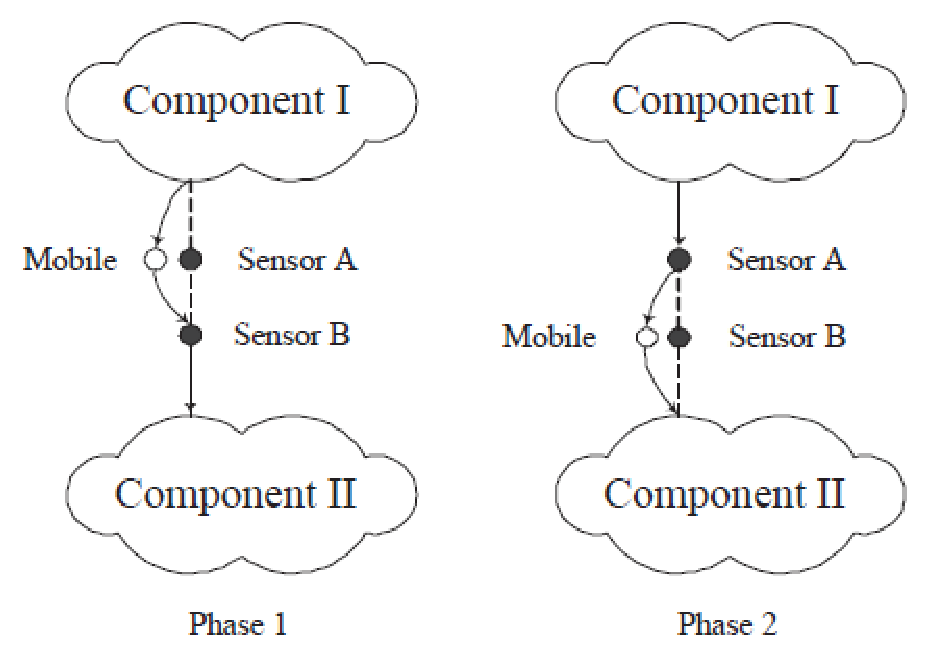
\includegraphics[width=0.6\textwidth]{images/mobile_help.eps}
	\caption{O κινητός κόμβος βοηθάει τους υπερφορτωμένους στατικούς κόμβους.}
	\label{fig:mobile_help}
\end{figure}
Ενα τέτοιο παράδειγμα φαίνεται στην εικόνα \ref{fig:mobile_help} (εξαγμένοι από το \cite{using_mobile_elements_to_prolong_lefetime}). Ολόκληρο το δίκτυο αποτελείται
από δύο μικρότερα υποδίκτυα ( Compnent I \& II) τα οποία είναι συνδεδεμένα μέσω των κόμβων Α και Β. Επομένως οι δύο αυτοί κόμβοι αποτελούν πέρασμα συμφόρησης αφού
πρέπει να προωθούν όλη την κίνηση από τα 2 υποδίκτυα. Ένας κινητός κόμβος μπορεί να προσομοιώσει την λειτουργία των Α και Β και έτσι να βελτιώσει τον χρόνο ζωής των
κόμβων αυτών και κατά συνέπεια του συνολικού δικτύου. Επίσης οι κινητοί κόμβοι μπορούν να συλλέξουν τα δεδομένα των στατικών κόμβων μέσω μικρής ακτίνα μετάδοσης
βοηθώντας στην εξοικονόμηση ενέργειας του κάθε κόμβου ξεχωριστά. Συγκεκριμένα, προκειμένου να μεγιστοποιηθεί ο χρόνος ζωής στο δίκτυο, ο κάθε στατικός κόμβος θα
πρέπει να στέλνει τα δεδομένα του σε έναν κινητό κόμβο αν και μόνο αν αυτός είναι σε απόσταση μικρότερης του ενός βήματος (hop). Ωστόσο, με αυτόν τον τρόπο υπάρχει
πολύ μεγάλη χρονοκαθυστέρηση (delay) στην μεταφορά των δεδομένων στην Πηγή. Από την άλλη μεριά αποστέλλοντας απευθείας στην Πηγή ή χρησιμοποιώντας πολυβηματικά
(multi-hop) πρωτόκολλα για την άμεση αναφορά γεγονότων στην Πηγή μειώνει δραστικά την χρονοκαθυστέρηση αλλά και τον χρόνο ζωής του δικτύου. Επομένως απαιτείται μία
χρυσή τομή ανάμεσα στην χρονοκαθυστέρηση και τον χρόνο ζωής του δικτύου που σίγουρα εξαρτάται από τον σκοπό και το περιβάλλον του δικτύου αισθητήρων.
\end{itemize}

Στη βιβλιογραφία έχουν χρησιμοποιηθεί πολλές διαφορετικές έννοιες για την περιγραφή των κινητών κόμβων στα ασύρματα δίκτυα αισθητήρων. Οι όροι διαφέρουν μεταξύ τους
ως προς το είδος και τον σκοπό του κινητού κόμβου. Για παράδειγμα κινητή Πηγή (mobile Sink ή mobile BS) χρησιμοποιείται για να περιγράψει μια κινητή Πηγή η οποία
έχει την δυνατότητα να περισυλλέγει δεδομένα από τους κοντινούς της κόμβους καθώς κινείται προκειμένου αυτοί να κάνουν πιο οικονομικές μεταδόσεις σε σχέση με μία
στατική Πηγή. Παρόμοια ο όρος κινητή οντότητα, ή πιο γενικά, κινητός κόμβος (mobile MULES, mobile entities, mobile relays) αναφέρεται σε κινητούς κόμβους οι οποίοι
έχουν παρόμοια υπολογιστική ισχύ όπως μια Πηγή και περιφέρονται σε όλο την περιοχή προκειμένου να περισυλλέξουν δεδομένα. Συχνά σε αυτό το μοντέλο είναι ότι
στο ασύρματο δίκτυο υπάρχει και μία Πηγή στην οποία οι κινητοί κόμβοι στέλνουν τα δεδομένα των στατικών κόμβων.

Επειδή η έρευνα σε αυτό τον τομέα των ασύρματων δικτύων αισθητήρων συνεχίζεται ακόμα και υπάρχει μεγάλο ενδιαφέρον στην πλήρη αξιοποίηση των κινητών κόμβων σε ένα
ΑΔΑ, θα παρουσιαστούν παρακάτω οι πιο σημαντικές εργασίες σε σχέση με την εκμετάλλευση κινητών Πηγών και κινητών κόμβων σε ένα δίκτυο αισθητήρων.

\subsection{Πρωτόκολλα με Κινητή Πηγή}
Η εργασία στο \cite{jointmobility} εξετάζει αν η κίνηση και η δρομολόγηση σε ένα δίκτυο αισθητήρων είναι φιλικές ή αλληλοσυγκρουόμενες έννοιες. Στο μοντέλο τους
εξετάζουν την περίπτωση ενός πυκνού δικτύου στο οποίο υπάρχουν στατικοί κόμβοι, τοποθετημένοι με μια Poisson κατανομή σε έναν κύκλο, έχουν μικρή ενέργεια και μια
κινητή Πηγή με άπειρη ενέργεια περιφέρεται στο δίκτυο προκειμένου να βοηθήσει στην δρομολόγηση και να περισυλλέξει τα δεδομένα όπως φαίνεται στην εικόνα
\ref{fig:jointmobility_model}.
\begin{figure}[h]
	\centering
	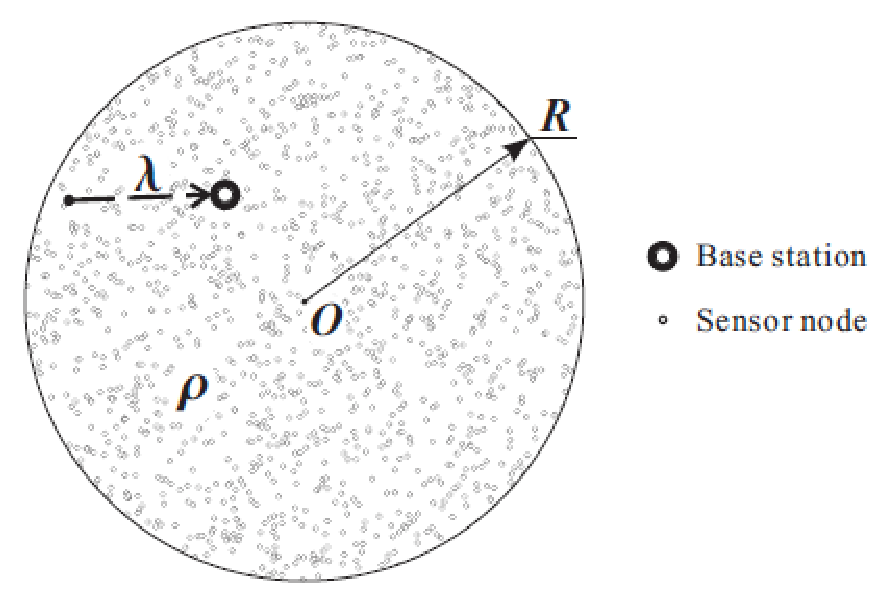
\includegraphics[width=0.6\textwidth]{images/jointmobility_model.eps}
	\caption{Κόμβοι τοποθετημένοι με Poisson κατανομή και Πηγή να κινείται στην περιφέρεια του κύκλου.}
	\label{fig:jointmobility_model}
\end{figure}
Οι συγγραφείς εξετάζουν την βέλτιστη θέση της Πηγής όταν αυτή είναι στατική και την βέλτιστη διαδρομή όταν αυτή είναι κινητή. Τελικά αποδεικνύουν ότι η βέλτιστη θέση
για την Πηγή όταν αυτή είναι στατική είναι το κέντρο του κύκλου. Αντίθετα όταν η Πηγή είναι κινητή αποδεικνύουν ότι η βέλτιστη διαδρομή της Πηγής είναι η περιφέρεια
του κύκλου. Αυτό συμβαίνει γιατί η διαδρομή αυτή είναι η μεγαλύτερη δυνατή που υπακούει και στην γεωμετρία του μοντέλου. Μια σύγκριση της εναπομείνασα ενέργειας με
τα προαναφερθέντα μοντέλα φαίνονται στην εικόνα \ref{fig:jointmobility_dissipation}.
\begin{figure}[h]
	\centering
	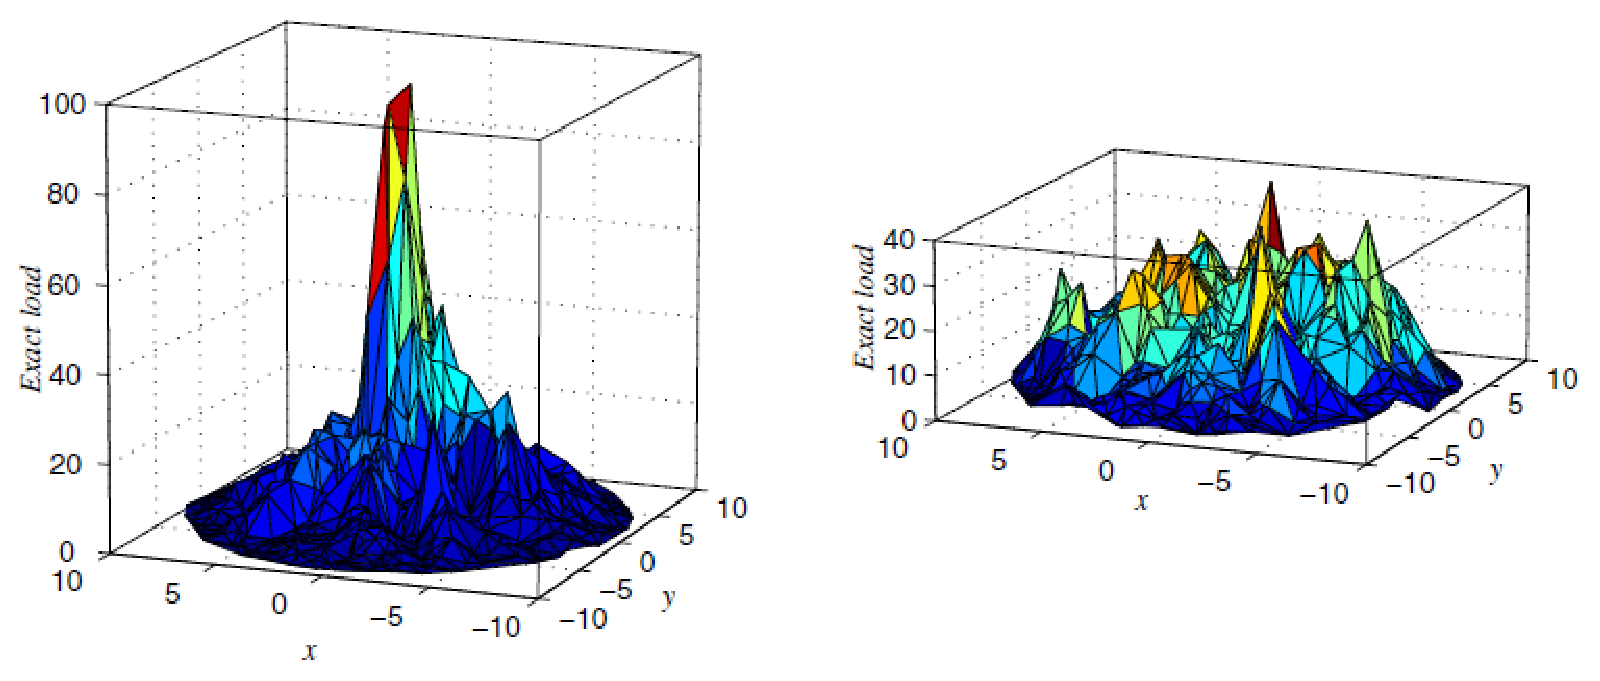
\includegraphics[width=\textwidth]{images/jointmobility_dissipation.eps}
	\caption{Ο ρυθμός κατανάλωσης της ενέργειας όταν η Πηγή είναι στο κέντρο του δικτύου(δεξιά) και όταν η κινείται στην περιφέρειά του(αριστερά).}
	\label{fig:jointmobility_dissipation}
\end{figure}

Όπως φαίνεται στην πρώτη εικόνα η στατική Πηγή δημιουργεί στους γύρω της κόμβους πολύ μεγάλους ρυθμούς κατανάλωσης ενέργειας. Αντίθετα, όταν η Πηγή είναι κινητή και
κινείται στην περιφέρεια του κύκλου, υπάρχει μεγαλύτερη εξισορρόπηση ενέργειας στο δίκτυο και επομένως αυξάνεται ο χρόνος ζωής του.
\begin{comment}

\end{comment}

Οι συγγραφείς παρουσίασαν μια ακόμη εργασία στο \cite{jointmobility_2006} ως συνέχεια της προηγούμενης στην οποία το μοντέλο είναι παρόμοιο με την προηγούμενη
εργασία και συγκρίνουν 2 περιπτώσεις για την αύξηση του χρόνου ζωής του δικτύου:
\begin{itemize}
\item \textbf{Γρήγορη κίνηση της Πηγής:} εξισορρόπηση της χρονοκαθυστέρησης (delay) με την κατανάλωση της ενέργειας
\item \textbf{Αργή κίνηση της Πηγής:} παροχή βοήθειας στους κρίσιμους κόμβους (bottleneck nodes)
\end{itemize}
Η αργή κίνηση της Πηγής επιτυγχάνεται μέσα από ένα γραμμικό πρόγραμμα
\begin{align*}
\text{Maximizing network lifetime } & T=\sum\limits_{i}T_{i}\\
\text{Constraints } & \sum\limits_{i}T_{i}P_{i}\leq E
\end{align*}
όπου $T_{i}$ ο χρόνος ζωής κάθε κόμβου, $P_{i}$ ο ρυθμός κατανάλωσης ενέργειας του κάθε κόμβου ως προς τον χρόνο και $E$ η συνολική ενέργεια του δικτύου.
Στην εργασία προτείνεται ένας αλγόριθμος 2 φάσεων ο οποίος χρησιμοποιεί το παραπάνω γραμμικό πρόγραμμα:
\begin{itemize}
\item \textbf{Αρχικοποίηση:} Κατά την αρχικοποίηση η κινητή Πηγή επισκέπτεται όλους τα σημεία-σταθμούς, συλλέγει τον ρυθμό κατανάλωσης κάθε σταθμού και κατασκευάζει
ένα προφίλ αυτού του σημείου-σταθμούς
\item \textbf{Εν λειτουργία:} Κατά την πραγματική λειτουργία η κινητή Πηγή παραμένει σε κάθε σημείο-σταθμό χρονικό διάστημα ανάλογο με τον ρυθμό κατανάλωσης της
ενέργειάς του.
\end{itemize}
Τα πειράματα αυτής της εργασίας έδειξαν ότι υπάρχει σημαντική αύξηση του χρόνου ζωής με τον αλγόριθμο των 2 φάσεων. Όμως ο αλγόριθμος δεν μπορεί να είναι
αποδοτικός και να επεκταθεί σε πολύ μεγάλα δίκτυα καθώς υπάρχει σημαντική καθυστέρηση.


Στην εργασία \cite{marios_randomwalks_1} αναλύεται η περίπτωση που υπάρχει κινητή Πηγή και αυτή κάνει έναν τυχαίο περίπατο (random walk). Γενικώς οι τυχαίοι
περίπατοι είναι πολύ εύκολοι στην υλοποίηση αφού χρησιμοποιούν μόνο τοπικές πληροφορίες και μπορούν να μειώσουν σημαντικά την κατανάλωση της ενέργειας λόγω της
τυχαιότητάς τους. Οι συγγραφείς προκειμένου να κάνουν ακόμα πιο αποδοτικούς τους τυχαίους περιπάτους, δημιουργούν τους προσαρμοστικούς τυχαίους περιπάτους. Σε αυτή
την περίπτωση, η κινητή Πηγή εκμεταλλεύεται κάποιες επιπλέον τοπικές πληροφορίες προκειμένου να επηρεάσει το επόμενο βήμα της, το οποίο και πάλι γίνεται πιθανοτικά
μόνο που αυτή τη φορά όχι τελείως ομοιόμορφα τυχαία αλλά προς την σωστότερη κατεύθυνση. Στο μοντέλο της εργασίας, η περιοχή του δικτύου χωρίζεται σε κελιά στα οποία
μόλις βρεθεί η κινητή Πηγή μέσα σε ένα από αυτά, γνωρίζει την κατάσταση όλων των αισθητήρων που ανήκουν στο ίδιο κελί. Οι συγγραφείς συγκρίνουν διάφορους τύπους
τυχαίων περιπάτων:
\begin{itemize}
\item \textbf{Τυφλός τυχαίος περίπατος:} Σε αυτή την περίπτωση η κινητή Πηγή επιλέγει ομοιόμορφα τυχαία μία από τις 4 κατευθύνσεις που θα ακολουθήσει στο επόμενο
βήμα. Αν και πιθανοτικά αυτή η λύση εγγυάται ότι η Πηγή θα φθάσει σε όλους τους κόμβους και όλα τα δεδομένα θα περισυλλεγούν, δημιουργεί σημαντικά προβλήματα
χρονοκαθυστέρησης. Για παράδειγμα η κινητή Πηγή μπορεί πολλές φορές να πηγαίνει σε σημεία τα οποία έχει ξαναεπισκεφθεί.
\item \textbf{Τυχαίος περίπατος με μνήμη:} Σε αυτή την περίπτωση η κινητή Πηγή θυμάται τα $Κ$ τελευταία κελιά τα οποία έχει επισκεφθεί κατά την διάρκεια του τυχαίου
περιπάτου της. Κάθε φορά το επόμενο βήμα επιλέγεται τυχαία με βάση τα κελιά τα οποία δεν ανήκουν στα $Κ$ τελευταία. Φυσικά υπάρχει ένας συμβιβασμός (trade off) ως
προς το μέγεθος του $K$. Για παράδειγμα αν το $K$ είναι πολύ μικρό, τότε η κινητή Πηγή ουσιαστικά εκτελεί τυχαίο περίπατο. Αντίθετα αν το $Κ$ είναι πολύ μεγάλο η
κινητή Πηγή μπορεί να βρεθεί σε κάποιο αδιέξοδο όταν για παράδειγμα όλα τα επόμενα δυνατά κελιά τα έχει ήδη επισκεφθεί.
\item \textbf{Τυχαίος περίπατος με αδράνεια:} Στην περίπτωση αυτή η πιθανότητα κάθε κατεύθυνσης του επόμενου βήματος προσαρμόζεται ανάλογα με την ανακάλυψη νέων
κόμβων. Συγκεκριμένα ο αλγόριθμος ενισχύει τις κατευθύνσεις στις οποίες εμφανίζονται καινούργιοι κόμβοι και αποδυναμώνει τις κατευθύνσεις στις οποίες υπάρχουν κόμβοι
που ήδη έχουν επισκεφθεί.
\item \textbf{Τυχαίος περίπατος explore n go:} Σε αυτή την περίπτωση η κινητή Πηγή ακολουθεί μία ευθεία γραμμή (δηλαδή προχωράει ίσια) όσο βρίσκει καινούργιους
κόμβους και αλλάζει κατεύθυνση αν βρεθούν κόμβοι που έχουν επισκεφθεί ή φθάσει στην άκρη του δικτύου. Ο τυχαίος περίπατος αυτός έχει παρόμοια απόδοση με τον τυχαίο
περίπατο με αδράνεια.
\item \textbf{Κατσαρός (curly) τυχαίος περίπατος:} Ο τυχαίος περίπατος αυτός παρομοιάζει την ντετερμινιστική σπείρα. Συγκεκριμένα η κινητή Πηγή ξεκινάει από μια
περιοχή και εκτελεί αριστερές στροφές οι οποίες μεγαλώνουν με τον χρόνο. Μετά από αρκετό διάστημα, ο τυχαίος περίπατος θα έχει καλύψει όλο το δίκτυο.
\end{itemize}

Οι προσομοιώσεις έδειξαν ότι οι προσαρμοστικοί τυχαίοι περίπατοι κινητών Πηγών έχουν πολύ καλύτερα αποτελέσματα όσον αφορά την περισυλλογή των δεδομένων από τους
κόμβους σε σχέση με τους τυχαίους περιπάτους.

Στην εργασία \cite{deploying_multiple_sinks_wsns} αναλύεται η βέλτιστη τοποθεσία μιας κινητής Πηγής σε πολυ-βηματικά (multi-hop) δίκτυα αισθητήρων. Συγκεκριμένα οι
συγγραφείς αναπτύσσουν αρχικά έναν καθολικό αλγόριθμο μέσα από γραμμικό προγραμματισμό. Αποδεικνύουν ότι το βέλτιστο σημείο στο οποίο θα πρέπει να πάει μια κινητή
Πηγή, προκειμένου να υπάρχει μείωση της κατανάλωσης της ενέργειας, είναι αυτό στο οποίο το άθροισμα όλων των διανυσμάτων κόμβου-Πηγής ισούται με το 0. Ουσιαστικά
πρόκειται για το γεωμετρικό κέντρο. Επειδή ο αλγόριθμος αυτός απαιτεί καθολικά (global) δεδομένα, οι συγγραφείς προτείνουν έναν αλγόριθμο που χρησιμοποιεί τοπικά
δεδομένα αλλά πετυχαίνει σχεδόν το ίδιο αποτέλεσμα με τον καθολικό αλγόριθμο. Στον τοπικό αλγόριθμο, κάθε κόμβος κρατάει στη μνήμη του τον αριθμό των μονοπατιών τα
οποία έχουν δημιουργηθεί από το πρωτόκολλο δρομολόγησης και περνάνε από μέσα του. Με αυτόν τον τρόπο η κινητή Πηγή χρειάζεται τα δεδομένα μόνο των πρώτων γειτόνων
της οι οποίοι θα έχουν σίγουρα αριθμό μονοπατιών μεγαλύτερο από τους πιο μακρινούς γείτονές της. Οι αριθμοί αυτοί προσομοιώνουν τα διανύσματα αποστάσεων που
αναφέρθηκαν νωρίτερα. Έτσι, αν ας κόμβος έχει μεγάλο αριθμό μονοπατιών, η Πηγή κινείται προς αυτό το σημείο προκειμένου να "ξεκουράσει" τον κόμβο. Στην εργασία αυτή,
οι συγγραφείς μελετάνε και την περίπτωση πολλών κινητών Πηγών.

\subsection{Πρωτόκολλα με Κινητούς Κόμβους} %nikoletsea's paper
Όπως και στην περίπτωση της μιας κινητής Πηγής στο δίκτυο αισθητήρων έτσι και στην περίπτωση πολλών κινητών Πηγών-κόμβων υπάρχει πολύ μεγάλη έρευνα. Αν και σε πολλές
εργασίες απλά επεκτείνεται η λογική της μίας κινητής Πηγής σε πολλές, η σωστή κατανομή των Πηγών καθώς και ο σωστός αριθμός των Πηγών αποτελούν χαρακτηριστικά προς
έρευνα.

Η εργασία στο \cite{data_mules} αποτελεί σημείο αναφοράς για τα δίκτυα αισθητήρων με κινητούς κόμβους. Στο μοντέλο θεωρείται ένα ΑΔΑ τριών επιπέδων. Στο κάτω επίπεδο
βρίσκονται οι στατικοί κόμβοι οι οποίοι επιβλέπουν το περιβάλλον. Στο αμέσως από πάνω επίπεδο βρίσκονται οι κινητοί κόμβοι οι οποίοι επισκέπτονται τους στατικούς
κόμβους προκειμένου να συλλέξουν πληροφορίες. Τέλος στο ανώτερο επίπεδο βρίσκονται τα σημεία πρόσβασης (ΣΠ ή access points) τα οποία ουσιαστικά αποτελούν Πηγές στις
οποίες παραδίδονται όλα τα δεδομένα των κινητών κόμβων. Επίσης θεωρείται ότι οι κινητοί κόμβοι θα πρέπει να φτάσουν σε απόσταση ενός βήματος (1-hop) ώστε να μπορούν
να επικοινωνήσουν με άλλους κόμβους ή σημεία πρόσβασης. Για την ανάλυση της απόδοσης, το δίκτυο χωρίζεται σε πλέγματα. Στην συνέχεια αποδεικνύεται ότι αν $\rho_{AP}$
είναι η πυκνότητα των σημείων πρόσβασης, η μέση τιμή του χρόνου που χρειάζεται ένας κινητός κόμβος να ξεκινήσει από ένα σημείο πρόσβασης και να ξανακαταλήξει σε αυτό
ή σε ένα άλλο κάνοντας τυχαίο περίπατο είναι $\frac{1}{\rho_{AP}}$. Επίσης, αποδεικνύεται ότι ο μέσος χρόνος που χρειάζεται να συναντήσει ένας κινητός κόμβος έναν
τυχαίο στατικό κόμβο είναι $\rho_{MULES}$ όπου $\rho_{MULES}$ είναι η πυκνότητα των κινητών κόμβων στο δίκτυο. Αντίστοιχα αποτελέσματα αποδεικνύονται για την πρώτη
επίσκεψη (hitting time) και την ποσότητα δεδομένων που αποθηκεύονται στη μνήμη των κόμβων αλλά και τον λόγο επιτυχίας των μηνυμάτων. Φυσικά όλα τα αποτελέσματα
αναφέρονται σε μέσες τιμές και προκειμένου να υπάρχει συγκέντρωση γύρω από την μέση τιμή θα πρέπει να εφαρμοστούν μέθοδοι που βασίζονται σε ροπές δεύτερης τάξης.
Ωστόσο, η ανάλυση που παρουσιάζεται σε αυτή την εργασία αποτελεί ένα καλό βοήθημα για την κατανόηση παρόμοιων μοντέλων.

Στην εργασία \cite{yuanyuan1} αναλύεται το πρόβλημα της τοποθέτησης κινητών κόμβων οι οποίοι θα λειτουργούν ως αρχηγοί σε συστάδες. Στο μοντέλο τους, παρουσιάζουν
μια αρχιτεκτονική τριών επιπέδων στην οποία στη βάση υπάρχουν οι στατικοί κόμβοι, μετά υπάρχουν οι κινητοί κόμβοι και τέλος υπάρχει η Πηγή. Θεωρούν ότι οι
κινητοί κόμβοι μπορούν να επικοινωνήσουν μεταξύ τους και με την Πηγή ώστε να της αποστείλουν τα τελικά δεδομένα. Αφού δείξουν ότι το πρόβλημα τοποθέτησης των κινητών
κόμβων στο δίκτυο ώστε να μεγιστοποιηθεί ο χρόνος ζωής του δικτύου είναι NP-hard (κάνοντάς το αναγωγή στο k-center πρόβλημα) παρουσιάζουν έναν ευρετικό αλγόριθμο που
λύνει το πρόβλημα αυτό σχετικά γρήγορα. Ο ευρετικός αλγόριθμος βασίζεται στην κατασκευή ενός χάρτη των ενεργειών των κόμβων της συστάδας μέσα από πληροφορίες των
κόμβων της ίδιας της συστάδας.


Η εργασία στο \cite{event_residual_hybrid} ακολουθεί μοντέλο παρόμοιο με την προηγούμενη. Οι συγγραφείς αναλύουν αρχικά από τι εξαρτάται ο χρόνος
ζωής ενός δικτύου και στην συνέχεια βασιζόμενοι στην ανάλυσή τους προτείνουν έναν υβριδικό αλγόριθμο. Όπως αποδεικνύουν ο χρόνος του δικτύου εξαρτάται από πολλούς
παράγοντες, οι πιο σημαντικοί από τους οποίους είναι: από την αρχική του ενέργεια, τον ρυθμό που παράγονται οι πληροφορίες, το μέγεθος του δικτύου, την ακτίνα
μετάδοσης ενός κόμβου αλλά και ενεργειακοί παράγοντες που αφορούν τα κυκλώματα του κάθε κόμβου για την λειτουργία των κυκλωμάτων. Παρουσιάζουν 2 στρατηγικές για τις
κινητές Πηγές που μπορούν να υπάρξουν. Στην πρώτη η κάθε κινητή Πηγή πηγαίνει στο σημείο μικρότερης ενέργειας της συστάδας της. Το πλεονέκτημα αυτής της στρατηγικής
είναι ότι δημιουργείται ένα πλήρως ενεργειακά ομοιόμορφο δίκτυο και επομένως αυξάνεται ο χρόνος ζωής του. Στην δεύτερη στρατηγική η κάθε κινητή Πηγή πηγαίνει ακριβώς
στο σημείο που παράγεται ένα γεγονός. Σε αυτή την περίπτωση η κινητή Πηγή λαμβάνει άμεσα τα δεδομένα από το γεγονός, το οποίο στο μοντέλο διαρκεί αρκετό χρονικό
διάστημα, έτσι ώστε τα δεδομένα δεν στέλνονται στους υπόλοιπους κόμβους και επομένως χάνεται ελάχιστη ενέργεια για την μεταφορά αυτών. Όμως η στρατηγική αυτή
δημιουργεί ανομοιογενή κατανομή ενέργειας στο δίκτυο. Ο υβριδικός αλγόριθμος που παρουσιάζουν οι συγγραφείς συνενώνει τις 2 στρατηγικές. Πειράματα έδειξαν
σημαντική βελτίωση του χρόνου ζωής του δικτύου.

Στην εργασία στο \cite{yuanyuan2} αναλύεται ξανά η βέλτιστη τοποθέτηση των κινητών Πηγών οι οποίες λειτουργούν ως αρχηγοί συστάδων όπως στο \cite{yuanyuan1} αλλά αυτή
τη φορά οι συγγραφείς στοχεύουν στην αποδοτική περισυλλογή δεδομένων. Αφού αποδείξουν ότι το πρόβλημα αυτό είναι NP-hard με αναγωγή στο TSP πρόβλημα, παρουσιάζουν τον
αλγόριθμό τους ο οποίος αποτελείται από 3 βήματα και παρουσιάζεται στην εικόνα \ref{fig:yuanyuan_mst}.
\begin{figure}[h]
	\centering
	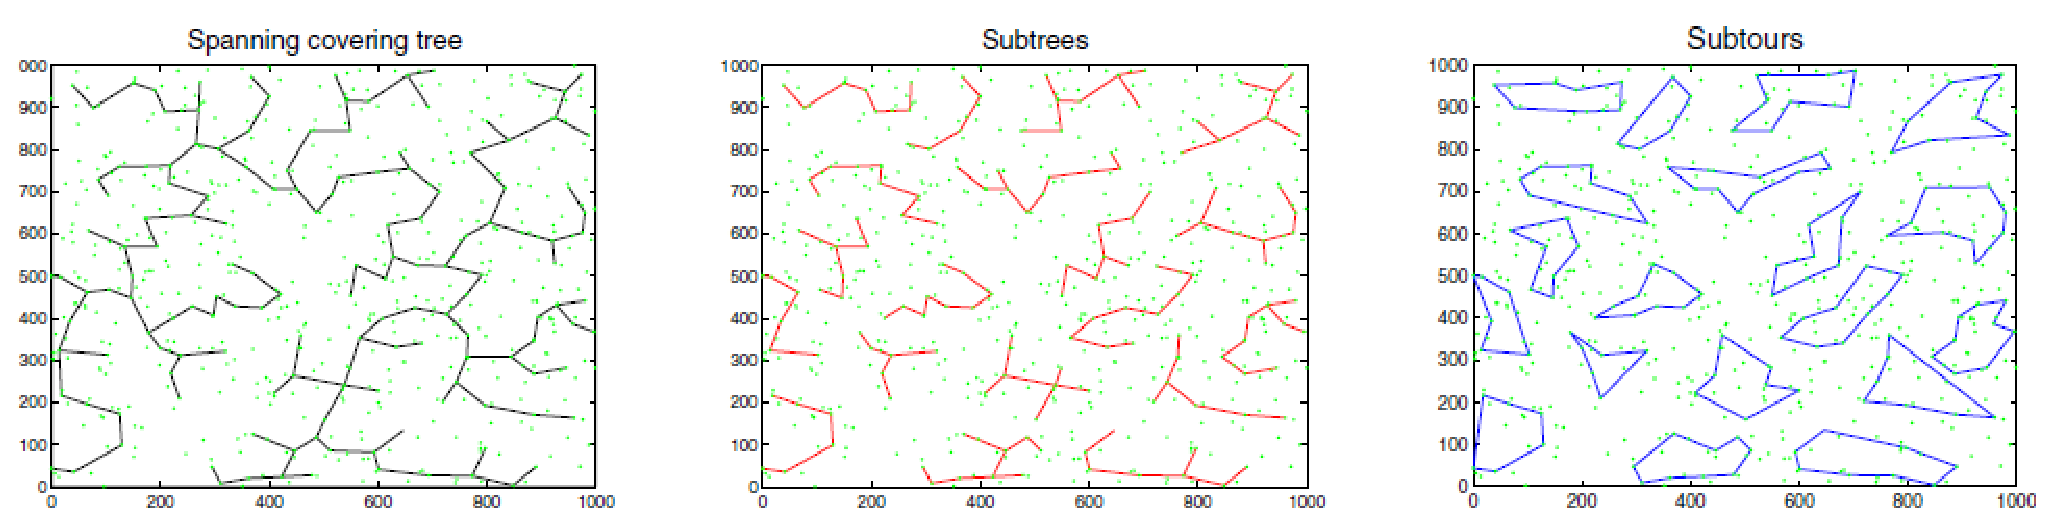
\includegraphics[width=\textwidth]{images/yuanyuan_mst.eps}
	\caption{Τα 3 βήματα του αλγορίθμου.}
	\label{fig:yuanyuan_mst}
\end{figure}
Αφού κατασκευαστεί κατανεμημένα ένα ελάχιστο γεννητικό δέντρο με όλους τους κόμβους, το δέντρο αυτό αποσυντίθεται σε μικρότερα ελάχιστα γεννητικά δέντρα, όσες και
οι κινητές Πηγές και αναζητείται σε κάθε τέτοιο δέντρο το μικρότερο μονοπάτι το οποίο επισκέπτεται όλους τους κόμβους. Οι κινητές Πηγές στέλνουν τα δεδομένα τους
στην κύρια Πηγή χρησιμοποιώντας της υπόλοιπες κινητές Πηγές. Πειράματα έδειξαν ότι εξοικονομείται σημαντικό ποσό της ενέργειας.


Η εργασία στο \cite{dynamic_deadlines} εξετάζει το πρόβλημα από μια διαφορετική σκοπιά. Οι συγγραφείς αρχικά επισημαίνουν ότι το πρόβλημα με τις κινητές Πηγές
ουσιαστικά πρόκειται για την δρομολόγηση κινητών με χρονικές προθεσμίες οι οποίες καθορίζονται από τον χώρο μνήμης ενός κόμβου ή πιο αφαιρετικά από το μέγιστο μέγεθος
των δεδομένων κάθε κόμβου θα κρατάει πριν τα παραδώσει στην Πηγή. Υπό αυτή την έννοια το πρόβλημα είναι λίγο διαφορετικό από το TSP πρόβλημα με την έννοια ότι η κάθε
κινητή Πηγή μπορεί να χρειαστεί να επισκεφθεί περισσότερες από μια φορά έναν κόμβο ανάλογα με τον ρυθμό παραγωγής των γεγονότων σε εκείνη την περιοχή. Αφού
αποδείξουν ότι το πρόβλημα είναι NP-complete κατασκευάζουν 3 ευρετικούς αλγορίθμους.
\begin{itemize}
\item \textbf{Νωρίτερη προθεσμία πρώτα:} σε αυτή την περίπτωση ο αλγόριθμος επισκέπτεται πρώτα τον κόμβο του οποίου ο χώρος μνήμης είναι πιο κοντά να ξεχειλίσει. Το
πρόβλημα με αυτόν τον ευρετικό αλγόριθμο είναι ότι δεν παίρνει υπόψιν του καθόλου το κόστος του κάθε κόμβου για να τον επισκεφθεί, δηλαδή την απόστασή του από την
τωρινή θέση της κινητής Πηγής.
\item \textbf{Νωρίτερη προθεσμία με $k$-κόμβους μπροστά:} σε αυτή την περίπτωση η κινητή Πηγή ταξινομεί τις προθεσμίες όλων των κόμβων και επιλέγει τις $k$
μικρότερες. Στη συνέχεια, επιλέγει την σειρά με την οποία θα επισκεφθεί τους $k$ αυτούς κόμβους έτσι ώστε καμία προθεσμία να μην χαθεί και ταυτόχρονα η συνολική
διαδρομή, δηλαδή ο χρόνος που θα χρειαστεί, να είναι η μικρότερη δυνατή.
\item \textbf{Ελάχιστο ζυγισμένο άθροισμα πρώτα:} σε μία προσπάθεια να εξισορροπήσουν το κόστος απόστασης με την χρονική προθεσμία οι συγγραφείς δημιούργησαν αυτόν
τον υβριδικό ευρετικό αλγόριθμος. Δηλαδή δημιουργούν το διάνυσμα
\begin{align*}
weighted\_sum[i] = & \alpha_{mwsf}\dot (deadline[i]-current\_time[i]) +\\
& (1-\alpha_{mwsf})(cost[current\_position][i])
\end{align*} και επιλέγουν τον κόμβο που έχει την μικρότερη τιμή.
\end{itemize}
Στην συνέχεια συγκρίνουν τους αλγορίθμους αυτούς με έναν αρκετά γνωστό
ευρετικό αλγόριθμο ο οποίος προέρχεται από την δρομολόγηση οχημάτων \cite{vehicle_routing_windows}. Τα βήματα του αλγορίθμου είναι τα εξής:
\begin{enumerate}
\item Ξεκινάει με ένα όχημα και έναν κόμβο ο οποίος είναι ο πρώτος στην διαδρομή του
\item Στην συνέχεια βρίσκει τον καλύτερο κόμβο που μπορεί να εισέλθει στην διαδρομή του
\begin{itemize}
	\item Αυτό συνεχίζεται μέχρι κανένας νέος κόμβος να μην μπορεί να εισέλθει λόγω περιορισμών στις προθεσμίες
\end{itemize}
\item Ο αλγόριθμος τότε προσθέτει ένα νέο όχημα και η διαδικασία συνεχίζεται παρόμοια για το νέο όχημα
\end{enumerate}
 Ο αλγόριθμος αυτός μπορεί να εφαρμοστεί και για την δρομολόγηση των κινητών Πηγών σε ένα ασύρματο δίκτυο αισθητήρων αφού τα 2 προβλήματα είναι παρόμοια.

Μια διαφορετική, ριζοσπαστική προσέγγιση εμφανίστηκε στην εργασία \cite{extending_lifetime_rizo}. Καταρχήν, το μοντέλο της εργασίας υποθέτει έναν κύκλο ακτίνας $R$
μέσα στον οποίο τοποθετούνται ομοιόμορφα κατανεμημένα $N$ κόμβοι. Επίσης όλοι ο κόμβοι οι οποίοι είναι 2-βήματα ή 1-βήμα ( 2-hop ή 1-hop) μακριά από την στατική Πηγή
ανήκουν στο σύνολο $G$. Στην εργασία αυτή οι συγγραφείς εκμεταλλεύονται τους κόμβους που ανήκουν στο $G$ "καίγοντάς" τους μέσα από έναν κινητό κόμβο.
\begin{figure}[h]
\begin{subfigure}{0.4\textwidth}
\centering
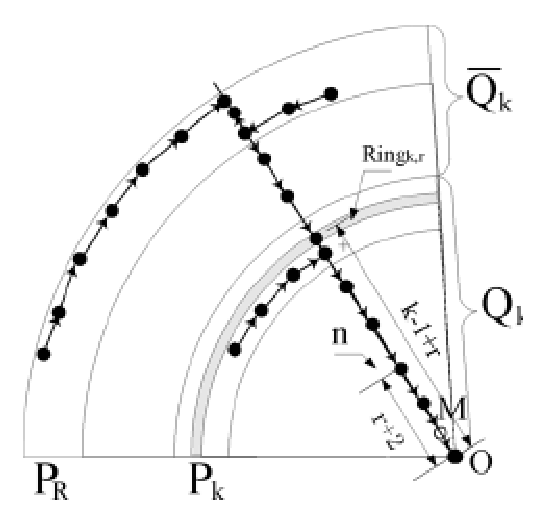
\includegraphics[scale=0.4]{images/extending_lifetime_1.eps}
\caption{}
\label{fig:extending_lifetime_path}
\end{subfigure}
\begin{subfigure}{0.5\textwidth}
\centering
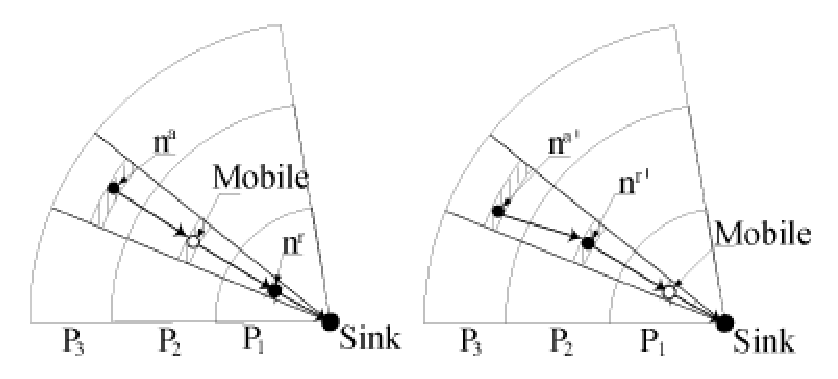
\includegraphics[scale=0.5]{images/extending_lifetime_2.eps}
\caption{}
\label{fig:extending_lifetime_depletion}
\end{subfigure}
\caption{Η διαδρομή που ακολουθούν τα πακέτα (α') και ο τρόπος που εκμεταλλεύεται τους 2-hop γείτονες της στατικής Πηγής ο κινητός κόμβος (β'). }
\label{fig:}
\end{figure}
Όπως φαίνεται και στην εικόνα \ref{fig:extending_lifetime_depletion} ο κινητός κόμβος αντικαθιστά κάθε φορά έναν κόμβο από αυτούς που είναι 2-βήματα ή 1-βήμα μακριά
και χρησιμοποιεί τον άλλον (ο οποίος βρίσκεται πάνω στην ακτίνα που σχηματίζεται από τον κινητό κόμβο και την στατική Πηγή έστω $r$) μέχρι να του εξαντλήσει τελείως
την ενέργειά του. Κάθε φορά που ο κινητός κόμβος επιλέγει έναν νέο κόμβο $u_{i}\in G$ τότε όλοι οι κόμβοι οι οποίοι ανήκουν στην ακτίνα $r$ λαμβάνουν όλα τα πακέτα
από όλους του κόμβους που ανήκουν στο ίδιο δαχτυλίδι. Δηλαδή οι κόμβοι που ανήκουν σε έναν δακτύλιο στέλνουν τα πακέτα τους πάνω από αυτόν δακτύλιο μέχρι να φτάσουν
στον κόμβο που ανήκει στην ακτίνα $r$ όπως φαίνεται και στην εικόνα \ref{fig:extending_lifetime_path}. Οι συγγραφείς αποδεικνύουν αναλυτικά ότι με αυτό το σχήμα το
δίκτυο μπορεί να έχει χρόνο ζωής  $T>4\frac{E}{R^{2}e}-\frac{16E}{R^{4}e}$ δεδομένου ότι για την ακτίνα του δικτύου $R$ ισχύει $R>16\pi+4$. Χρησιμοποιώντας την ίδια
λογική αποδεικνύεται ότι για $m$ κινητούς κόμβους (οι οποίοι εκμεταλλεύονται $2m$ στατικούς κόμβους πάνω στην ακτίνα $r$) ο χρόνος ζωής του δικτύου φράσσεται από την
σχέση:
\begin{align*}
T>4m\frac{E}{R^{2}e}-\frac{32\pi m^{3}E}{R^{4}e} \qquad\text{αν η ακτίνα $R$ είναι αρκετά μεγάλη}
\end{align*}
Τα πειράματα αυτής της εργασίας έδειξαν ότι ο χρόνος ζωής αυξάνεται σημαντικά και επαληθεύονται τα προηγούμενα θεωρητικά αποτελέσματα. Όπως έγινε εμφανές η εργασία
αυτή ακολουθεί μια διαφορετική λογική από τις υπόλοιπες σχετικές εργασίες το οποίο την κάνει ξεχωριστή.

Μια επίσης διαφορετική εργασία στο \cite{auction_energy_balance}. Στην εργασία αυτή θεωρείται ένα υβριδικό δίκτυο αισθητήρων το οποίο αποτελείται από κινητούς
κόμβους και στατικούς κόμβους. Στο μοντέλο θεωρείται ότι οι κινητοί κόμβοι έχουν πολύ περισσότερη ενέργεια από τους στατικούς, ο χρόνος χωρίζεται σε γύρους και η
εργασία επικεντρώνεται στην κατάλληλη διαχείριση των κινητών κόμβων σε έναν γύρο. Να σημειωθεί ότι αποτελεί από τις λίγες εργασίες που παίρνει υπόψιν στο μοντέλο της
και στοχεύει στην μείωση της κατανάλωσης την ενέργεια που σπαταλάται για την κίνηση ενός κινητού κόμβου. Οι συγγραφείς προτείνουν αρχικά έναν καθολικό (centralized)
αλγόριθμο και στην συνέχεια έναν κατανεμημένο αλγόριθμο. O κατανεμημένος αλγόριθμος χρησιμοποιεί μια διαφορετική προσέγγιση για να λύσει το πρόβλημα της
δρομολόγησης των κινητών κόμβων. Αρχικά η περιοχή του δικτύου χωρίζεται σε ένα πλέγμα (grid) και κάθε κελί εκλέγει έναν στατικό κόμβο ως αρχηγό. Ο χρόνος χωρίζεται
περαιτέρω σε 3 διαφορετικές φάσεις ενός γύρου:
\begin{itemize}
\item \textbf{Φάση διάδοσης:} Αρχικά ο αρχηγός κάθε κελιού μέσα στο πλέγμα συλλέγει τις τοποθεσίες των γεγονότων από τους στατικούς αισθητήρες. Επίσης συλλέγει τις
αναφορές (τοποθεσία, ενέργεια) των κινητών κόμβων. Στην συνέχεια η ύπαρξη των κινητών κόμβων διαφημίζεται από τα κελιά που τους περιέχουν.
\item \textbf{Φάση διαγωνισμού:} Κάθε κελί του πλέγματος που περιέχει ένα γεγονός (και επομένως πρέπει να έρθει ένας κινητός κόμβος για να το συλλέξει) διαγωνίζεται
με όλα τα άλλα αντίστοιχα κελιά για τους κινητούς κόμβους χρησιμοποιώντας προσκλήσεις. Ο κάθε κινητός κόμβος αποδέχεται ή απορρίπτει μια πρόσκληση ανάλογα με τα
δεδομένα της πρόσκλησης όπως π.χ η απόσταση του γεγονότος από τη θέση του κινητού κόμβου.
\item \textbf{Φάση δρομολόγησης:} Ο κάθε κινητός κόμβος αφού έχει επιλέξει μια σειρά από κελιά τότε εκτελεί την διαδρομή του χρησιμοποιώντας προσεγγιστικό αλγόριθμο
του προβλήματος TSP.
\end{itemize}
Αποδεικνύεται ότι η πολυπλοκότητα του αλγορίθμου είναι $O(m\cdot\hat{M} + n\cdot\hat{N} + m^{2}h)$ όπου $m,n$ οι κινητοί και στατικοί κόμβοι αντίστοιχα, $\hat{M},
\hat{N}$ οι διαστάσεις του πλέγματος και $h$ η διάμετρος του δικτύου. Οι προσομοιώσεις δείξαν ότι υπάρχει σημαντική αύξηση του χρόνου ζωής του δικτύου.



\section{Εναλλακτικές Τεχνικές} % node density(normal distribution)
Εκτός από τους αλγόριθμους δρομολόγησης υπάρχουν και άλλες τεχνικές που έχουν μελετηθεί με σκοπό την επέκταση του χρόνου ζωής ενός ασύρματου δικτύου αισθητήρων.
Έχουν μελετηθεί τεχνικές που έχουν να κάνουν με αξιοποίηση εναλλακτικών πηγών ενέργειας όπως είναι η ηλιακή ενέργεια αλλά και τεχνικές που θεωρούν πιο ισχυρά μοντέλα
όπως η πρόσθεση επιπλέον κόμβων σε ένα δίκτυο εκεί που χρειάζεται. Τέλος παρουσιάζεται μια νέα πρωτοπόρα ριζοσπαστική τεχνική, αυτή της ασύρματης
φόρτισης, η οποία αναλύεται εκτενέστερα στο κεφάλαιο \ref{ch:wrsns}.

\subsection{Τεχνικές εναλλακτικών πηγών ενέργειας}
Οι τεχνικές αυτές ασχολούνται με την αξιοποίηση εναλλακτικών πηγών ενέργειας (energy harvesting) προκειμένου να φορτίσουν τους στατικούς κόμβους που επιβλέπουν το
περιβάλλον. Τα τελευταία χρόνια αυτές οι τεχνικές έχουν γνωρίσει μεγάλη ανάπτυξη και έχουν ενσωματωθεί επιτυχημένα σε συστήματα ΑΔΑ. Υπάρχει ποικιλία διαφορετικών
ενεργειών που μπορούν να χρησιμοποιηθούν για την αύξηση ζωής του δικτύου όπως μηχανική, θερμική και ηλιακή ενέργεια κάθε μία από τις οποίες μπορεί να μετατραπεί σε
ηλεκτρική και να
ενεργοποιήσει τους κόμβους ή απλώς να επαναφορτίσει τις μπαταρίες τους. Η πιο πολυχρησιμοποιούμενη είναι η ηλιακή ενέργεια. Για την ηλιακή ενέργεια ο ρυθμός
επαναφόρτισης ορίζεται από τον παρακάτω τύπο:
\begin{align*}
\pi_{r} = Rad_{s} \times \eta_{\rho} \times \rho_{e} \times A
\end{align*}
όπου to $Rad_{s}$ αντιστοιχεί στην ηλιακή ακτινοβολία, το $\eta_{\rho}$ αντιστοιχεί στην αποδοτικότητα του ηλιακού συλλέκτη να μετατρέψει την ηλιακή ενέργεια σε
ηλεκτρική ενέργεια, το $\rho_{e}$ αντιστοιχεί στην απόδοση του ηλεκτρικού κυκλώματος και το $A$ αντιστοιχεί στο μέγεθος του ηλιακού συλλέκτη.

Ωστόσο καθώς όλες αυτές οι εναλλακτικές ενέργειες προέρχονται από το εξωτερικό περιβάλλον οι χωροχρονικοί χαρακτήρες τους έχουν μεγάλες διακυμάνσεις όσον αφορά την
απόδοση τους η οποία συνήθως είναι χαμηλή και ευαίσθητη στην δυναμική του περιβάλλοντος. Για παράδειγμα σε ένα σύστημα βασισμένο στην ηλιακή ενέργεια, η ισχύς εξόδου
του η οποία θα τροφοδοτήσει έναν αισθητήρα καθορίζεται από τις ηλιακές ακτίνες που προσάπτονται εκείνη την στιγμή στους ηλιακούς συλλέκτες και μεταβάλλεται σημαντικά
ανάλογα με την ώρα και τον καιρό. Στατιστικές έχουν δείξει ότι υπάρχει διαφορά μέχρι και 3 τάξεις μεγέθους στην διαθέσιμη ενέργεια ανάμεσα σε μια σκιώδη,
συννεφιασμένη και ηλιόλουστη μέρα \cite{harvesting_comparison}. Καθώς δεν υπάρχει γενικά τρόπος να γνωρίζει εξαρχής κανείς την κατάσταση που θα υπάρχει στο δίκτυο
αισθητήρων υπάρχει μεγάλη δυσκολία στο σχεδιασμό πρωτοκόλλων που εκμεταλλεύονται τέτοιες μορφές ενέργειας και να κρατάνε τους κόμβους πάντα ενεργούς. Αυτό όμως είναι
πολύ δύσκολο ειδικά σε εφαρμογές στις οποίες το κύριο έργο είναι να συλλέγουν περιοδικά δεδομένα και πληροφορίες από όλους τους κόμβους. Στην περίπτωση που κάποιοι
αισθητήρες καταναλώσουν όλη την ενέργειά τους και δεν επαναφορτιστούν γρήγορα, το δίκτυο σταδιακά θα καταρρεύσει. Υπάρχουν όμως πρωτόκολλα που ρυθμίζουν τις
λειτουργίες του κάθε κόμβου ανάλογα με την κατάσταση που επικρατεί στο εξωτερικό του περιβάλλον και παρουσιάζονται στην συνέχεια.

Μία από τις πρώτες εργασίες παρουσιάζεται στο \cite{heliomote}. Στην εργασία αυτή παρουσιάζεται ένα σύστημα του οποίου οι κόμβοι έχουν ηλιακούς συλλέκτες
και μπορούν να φορτίζονται από την ηλιακή ενέργεια όπως φαίνεται στην εικόνα \ref{fig:heliomote_example}.
\begin{figure}[h]
	\centering
	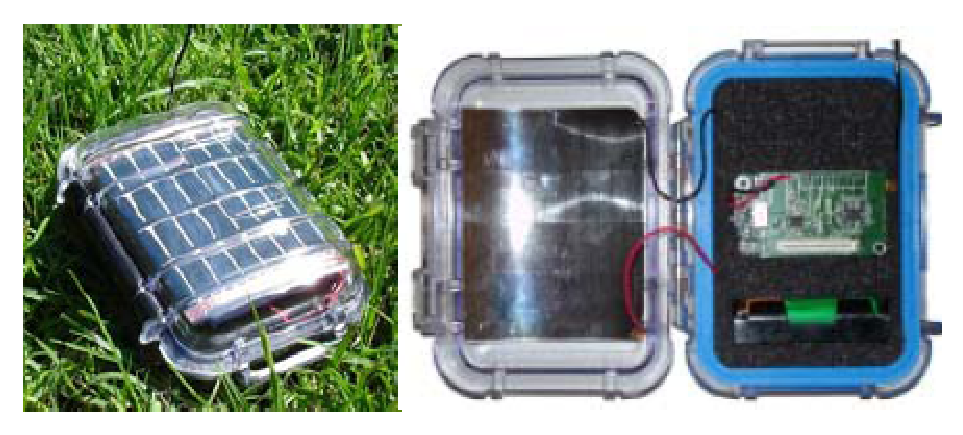
\includegraphics[width=0.8\textwidth]{images/heliomote_example.eps}
	\caption{Ένας κόμβος του συστήματος \textit{Heliomote}.}
	\label{fig:heliomote_example}
\end{figure}
Με αυτόν τον τρόπο το σύστημα μπορεί να επιμηκύνει το χρόνο ζωής του συλλέγοντας ενέργεια από τον ήλιο. Επιπλέον στην εργασία προτείνεται ένας εναλλακτικός τρόπος
δρομολόγησης των πακέτων. Συγκεκριμένα, τα πακέτα δρομολογούνται μέσα από μονοπάτια τα οποία έχουν το μεγαλύτερη συλλογή ηλιακής ενέργειας. Επίσης κόμβοι οι οποίοι
έχουν μικρή συλλογή ηλιακής ενέργειας (π.χ. είναι κάτω από ένα δέντρο) τότε μειώνουν τον φόρτο εργασίας τους εσκεμμένα. Υπάρχει επομένως εξισορρόπηση της ενέργειας
του δικτύου.

Στην εργασία \cite{harvesting_6} μελετάται η περίπτωση ενός ασύρματου δικτύου αισθητήρων στο οποίο υπάρχει πλεονασμός κόμβων οι οποίοι μπορούν να
επαναφορτιστούν. Η εργασία αναλύει το πρόβλημα του πως οι κόμβοι θα έπρεπε να ενεργοποιούνται δυναμικά έτσι ώστε να μεγιστοποιηθεί η κάλυψη του δικτύου. Αφού δειχθεί
η βέλτιστη λύση, στην συνέχεια προτείνεται μια κατανεμημένη πολιτική ενεργοποίησης η οποία επιτυγχάνει το $\frac{3}{4}$ της βέλτιστης λύσης ενώ παρέχονται
προσομοιώσεις που επιβεβαιώνουν τα θεωρητικά αποτελέσματα.

Στην εργασία \cite{harvesting_7} αναλύεται η απόδοση πολυ-βηματικών (multi-hop) μεταδόσεων στην περίπτωση που υπάρχει δυνατότητα επαναφόρτισης ορισμένων κόμβων. Στην
συνέχεια σχεδιάζεται ένας αλγόριθμος ο οποίος λαμβάνει υπόψιν του την αναπλήρωση ενέργειας των κόμβων και προωθεί τα πακέτα προς αυτούς τους κόμβους ο οποίος είναι
ασυμπτωτικά βέλτιστος σε αντιστοιχία με το μέγεθος του δικτύου. Ο αλγόριθμος δεν θεωρεί κάποια στατιστική πληροφορία όσον αφορά την άφιξη των πακέτων και επομένως
μπορεί να ενσωματωθεί σε ήδη υπάρχοντα σχήματα δρομολόγησης (προληπτικά ή κατ'απαίτηση). Τα αποτελέσματα των προσομοιώσεων επιβεβαίωσαν ότι ο αλγόριθμος πετυχαίνει
να μεγιστοποιήσει την απόδοση σε ενεργειακά (energy-aware) δίκτυα.

Στις εργασίες \cite{harvesting_8} \cite{harvesting_9} αναλύεται ξανά η βέλτιστη δειγματοληψία των κόμβων κάτω από τους περιορισμούς των εναλλακτικών ενεργειών όπως
είναι η φωτεινότητα στην ηλιακή ενέργεια. Σε κάθε περίπτωση προτείνεται ένας κατανεμημένος αλγόριθμος ο οποίος ρυθμίζει κατάλληλα τον ρυθμό δειγματοληψίας του κάθε
κόμβου και λύνει το πρόβλημα αποδοτικά. Τέλος εκτελούνται προσομοιώσεις που αποδεικνύουν την απόδοση του εκάστοτε αλγορίθμου.



\subsection{Τεχνικές αύξησης των κόμβων του δικτύου}
Στην τεχνική αυτή υπάγονται εργασίες οι οποίες αναλύουν την βέλτιστη κατανομή των κόμβων σε ένα ασύρματο δίκτυο αισθητήρων και εργασίες που προτείνουν αποδοτικούς
τρόπους για την αντικατάσταση κόμβων του δικτύου οι οποίοι έχουν χάσει πλήρως την ενέργειά τους. Στην πρώτη περίπτωση εκτελείται ένας προληπτικός αλγόριθμος (offline
algorithm) ο οποίος βρίσκει την βέλτιστη ανάπτυξη των αισθητήρων κάτω από συγκεκριμένες συνθήκες. Στη δεύτερη περίπτωση εκτελούνται αλγόριθμοι άμεσης
απόκρισης (online algorithms) οι οποίοι αφού αναλύσουν την κατάσταση του δικτύου, βρίσκουν το βέλτιστο υποσύνολο του δικτύου το οποίο θα πρέπει να αντικατασταθεί ή
να προστεθούν επιπλέον κόμβοι.

Στην εργασία \cite{gaussian_sensors} οι συγγραφείς αναλύουν την περίπτωση όπου οι κόμβοι δεν τοποθετούνται ομοιόμορφα κατανεμημένα αλλά με βάση την Gaussian κατανομή
σε δισδιάστατο χώρο. Στην συνέχεια εντοπίζουν κάτω από ποιες συγκεκριμένες υποθέσεις και ιδιότητες της Gaussian κατανομής μπορεί να επιτευχθεί η επιθυμητή κάλυψη και
διάρκεια ζωής του δικτύου. Αφού αναλύσουν τις στρατηγικές ανάπτυξης των κόμβων προτείνουν 2 αλγόριθμους ανάπτυξης των κόμβων οι οποίοι αυξάνουν σημαντικά τον χρόνο
ζωής του δικτύου.

Η εργασία στο \cite{sens_deployment3} εισάγει για πρώτη φορά στο μοντέλο των ΑΔΑ την έννοια της πρόσθεσης ή αντικατάστασης κόμβων του δικτύου ενώ ενσωματώνει στο
μοντέλο την έννοια της ετερογένειας, της ύπαρξης δηλαδή διαφορετικών κόμβων ως προς τις δυνατότητές τους. Με τις προαναφερθείσες παραδοχές αυξάνεται σημαντικά η
δυναμικότητα του δικτύου που μελετάται και οι συγγραφείς διαπιστώνουν ότι ο μόνος τρόπος για την αποδοτική διαχείριση της ενέργειας είναι μέσα από αλγόριθμους
μάθησης. Συγκεκριμένα, οι συγγραφείς αναπτύσσουν έναν κατανεμημένο αλγόριθμο ελαχιστοποίησης της ενέργειας ο οποίος χρησιμοποιεί τοπικές πληροφορίες όπως για
παράδειγμα πυκνότητα και ενέργεια του δικτύου σε μια τοπική περιοχή και ρυθμίζει κατάλληλα την πολιτική ύπνου (sleeping policy) των κόμβων. Οι προσομοιώσεις δείξαν
ότι με αυτόν τον τρόπο διπλασιάζεται σχεδόν ο λόγος επιτυχίας σε σύγκριση με το Directed Diffusion ενώ μαζί με την προσθήκη ετερογενών κόμβων σε κατάλληλα σημεία του
δικτύου ο λόγος επιτυχίας αυξάνεται ακόμα περισσότερο με παρόμοια ενεργειακή συμπεριφορά.

Η εργασίες στα \cite{sens_deployment1} \cite{sens_deployment2} μελετάνε την περίπτωση ενός δικτύου το οποίο λειτουργεί για πολύ μεγάλο χρονικό διάστημα. Για να
λύσουν το πρόβλημα που δημιουργείται από τους περιορισμένους πόρους ενέργειας που έχει ο κάθε κόμβος προτείνουν μια στρατηγική αντικατάστασης και ανάκτησης των παλιών
κόμβων με καινούργιους. Για την υλοποίηση της ιδέας χρησιμοποιείται ένα μηχανικά κινούμενο ρομπότ το οποίο έχει την ικανότητα να αντικαθιστά τους κόμβους του
δικτύου. Το ρομπότ αυτό περιοδικά διασχίζει την περιοχή του δικτύου και εγκαθιστά καινούργιους κόμβους ενώ επιστρέφει τους παλιούς κόμβους στην βάση για επαναφόρτηση.


\subsection{Τεχνικές επαναφόρτισης κόμβων} \label{sc:recharg_tecnhiques}
Η πρόσφατη πρόοδος στις περιοχές των υλικών που χρησιμοποιούνται για τις μπαταρίες αλλά και στην περιοχή της ασύρματης μετάδοσης ενέργειας προσφέρουν νέες δυνατότητες
διαχείρισης της διαθέσιμης ενέργειας. Στην πρώτη περιοχή ανακαλύφθηκε ένα νέο υλικό για μπαταρίες το οποίο επιτρέπει πολύ γρήγορες φορτίσεις και αργές αποφορτίσεις
\cite{fast_recharging}. Η ανακάλυψη αυτή συνδυάζει τα πλεονεκτήματα των κλασσικών $Li-ion$ μπαταριών και των υπερ-πυκνωτών χρησιμοποιώντας την τεχνολογία
$LiFePO_{4}$ επιτρέποντας φορτίσεις μέχρι και 400C\footnote{C ορίζεται ως η ονομαστική χωρητικότητα της μπαταρίας. Για παράδειγμα για μία
μπαταρία χωρητικότητας 1000mAh C=1000mA.}. Στη δεύτερη περιοχή η τεχνολογία γύρω από την ασύρματη μετάδοση ενέργειας έχει εξελιχθεί τόσο πολύ που πλέον τα ποσοστά
επιτυχίας έχουν ανέβει σημαντικά. Οι εργασίες στα \cite{wireless_recharg1}, \cite{wireless_recharg2}, \cite{wireless_recharg3} δείχνουν ότι μπορεί να υπάρξει μέχρι
και 60\% απόδοση στην μεταφορά ενέργειας. Ταυτόχρονα η Intel\textsuperscript{\textregistered} δείχνει μέχρι και 75\% απόδοση \cite{intel_recharg} ενώ η εταιρεία
Witricity\textsuperscript{\textregistered} ισχυρίζεται ότι μπορεί να επιτύχει μεταφορά ενέργειας με ποσοστό επιτυχίας μέχρι και 90\% \cite{witricity_90}. Η
συγκεκριμένη τεχνολογία έχει οδηγήσει σε έναν καινούργιο κλάδο των ασύρματων δικτύων αισθητήρων: τα ασύρματα επαναφορτιζόμενα δίκτυα αισθητήρων (ΑΕΔΑ). Θα αναλυθεί
εκτενέστερα στο επόμενο κεφάλαιο αφού αποτελεί τον κινητήριο μοχλό για αυτή την διπλωματική εργασία.
























